\chapter{Reading the Paper V: Discussion, Limits, and How to Go Further}\label{ch:paper-critique}

\begin{chapterintro}
You have now followed the paper~\cite{soniR1} from its question and protocol (Chapter~\ref{ch:paper-setup}), through its negative result on fitted potentials (Chapter~\ref{ch:paper-memorization}) and its positive result on the explicit formula (Chapter~\ref{ch:paper-arithmetic}), to its dissection of a spurious in-sample floor (Chapter~\ref{ch:paper-spurious-floor}). This last chapter does three things that a careful reader of any research paper should do once the results are understood.

First, it reads the Discussion (Sec.~VI of the paper) sentence by sentence. For each statement it asks what kind of statement it is: a numerical observation, a heuristic explanation, a proposal, or an open problem. Second, it plays referee. It lists the limits the paper states about itself, and then the weak points a skeptical expert could press, and for each it does a small calculation to see how much weight the point carries. Third, it shows you how to rerun the paper's anchor numbers yourself with the \texttt{qmnt} library and the Zenodo record~\cite{zenodo}, and it proposes graded research projects that start where the paper stops.

No new mathematics is introduced. Every tool you need was built in Parts I--V; we only combine those tools in small, honest calculations (probabilities of chance coincidences, worst-case phase errors, coverage thresholds) that help you judge the evidence.

\textbf{Where this shows up in the paper:} Sec.~VI (Discussion), Appendix~A (the reconstruction record, steps 1--23, the literature audit and the key anchors), the Data Availability statement, Sec.~II~F (use of artificial intelligence), and the hedges written into the captions of Tables~I--V.
\end{chapterintro}

\begin{prerequisites}
\item All of Parts I--V. In particular: the counting function $\Nsm$, smooth zeros and mean spacings (Chapter~\ref{ch:counting-zeros}); the truncated explicit formula (Chapter~\ref{ch:explicit-formula}); the Wu--Sprung potential and its turning points (Chapters~\ref{ch:wkb} and~\ref{ch:wu-sprung}); second-order non-Hermitian shifts (Chapter~\ref{ch:non-hermitian}); the finite-difference solver and bias correction (Chapter~\ref{ch:finite-differences}); fitting and the coverage law (Chapter~\ref{ch:fitting}); held-out testing and nulls (Chapter~\ref{ch:generalization}); bootstrap and surrogates (Chapter~\ref{ch:controls}); sparse frequency learning and dephasing (Chapter~\ref{ch:sparse-frequency}); correlation, independence and the Poisson law (Chapters~\ref{ch:probability} and~\ref{ch:level-statistics}); the prime number theorem (Chapter~\ref{ch:primes}).
\item Chapters~\ref{ch:paper-setup}--\ref{ch:paper-spurious-floor}, which read Secs.~I--V of the paper.
\item First-year physics: the habit of checking a claim by an order-of-magnitude estimate.
\end{prerequisites}

%======================================================================
\section{What the Discussion section claims}\label{sec:paper-critique-claims}

Before we judge anything we recall the vocabulary. The nontrivial zeros of the zeta function are $\rho_n=\tfrac12+it_n$, and $t_n>0$ is the height of the $n$-th zero. The smooth zeros $s_n$ solve $\Nsm(s_n)=n-\tfrac12$, where $\Nsm(t)=\frac{t}{2\pi}\log\frac{t}{2\pi}-\frac{t}{2\pi}+\frac78$ is the smooth counting function of paper Eq.~(1) (Chapter~\ref{ch:counting-zeros}). The local mean spacing is $\gap_n=ds_n/dn$. The \emph{fluctuation} of a zero is $(t_n-s_n)/\gap_n$, its displacement from the smooth zero measured in mean spacings. A \emph{prediction} $t^{\rm pred}_n$ has its own fluctuation $(t^{\rm pred}_n-s_n)/\gap_n$. The paper scores a prediction on a set of held-out (out-of-sample, OOS) zeros by two numbers: the rms, the root mean square of the error in units of mean spacing, and corr, the Pearson correlation of predicted with true fluctuations (Chapter~\ref{ch:probability}). The \emph{null} is the prediction ``no fluctuation'', $t^{\rm pred}_n=s_n$ (or, for the operator, the levels of the unperturbed Wu--Sprung potential). Since the null error of zero $n$ is the true fluctuation itself, the null rms is the rms of the true fluctuations; on the principal holdout, zeros 401--500 (running example RE5), it is $0.263$ (paper Sec.~II~C; anchor $0.2631$ in App.~A).

Sec.~VI of the paper has five paragraphs. We take them in order.

\subsection{Paragraph 1: the scope}

The Discussion opens: ``Nothing here touches the analytic Hilbert--P\'olya program''. What is constrained is ``a shortcut: the idea that flexible operator families fitted to finitely many zeros capture transferable spectral structure.''

\emph{In plain words.} The Hilbert--P\'olya conjecture (Chapter~\ref{ch:hilbert-polya}) hopes for a self-adjoint operator whose eigenvalues are the $t_n$. It is open. The paper does not test any operator that was written down \emph{before} looking at the zeros (such as the Berry--Keating, Connes, or Bender--Brody--M\"uller proposals~\cite{berrykeating99,connes,bbm}). It tests only a shortcut: take a flexible family of potentials, tune its parameters until its levels match the first few hundred zeros, and hope the tuned potential ``knows'' something about the zeros you did not show it.

\emph{Tools.} The distinction between analytic and empirical programs is Chapter~\ref{ch:hilbert-polya}; the meaning of ``transferable'' is the held-out test of Chapter~\ref{ch:generalization}.

\emph{Computation behind it.} The scoreboard of \cref{fig:paper-critique-scoreboard} collects the held-out rms on zeros 401--500 from paper Tables~I, IV and V. The fitted operators sit at or above the null line; every model that uses the arithmetic structure, given or learned, sits below it, and all but the underdetermined, root-ambiguous B row ($0.180$, Table~IV) sit far below it.

\begin{figure}[htbp]\centering
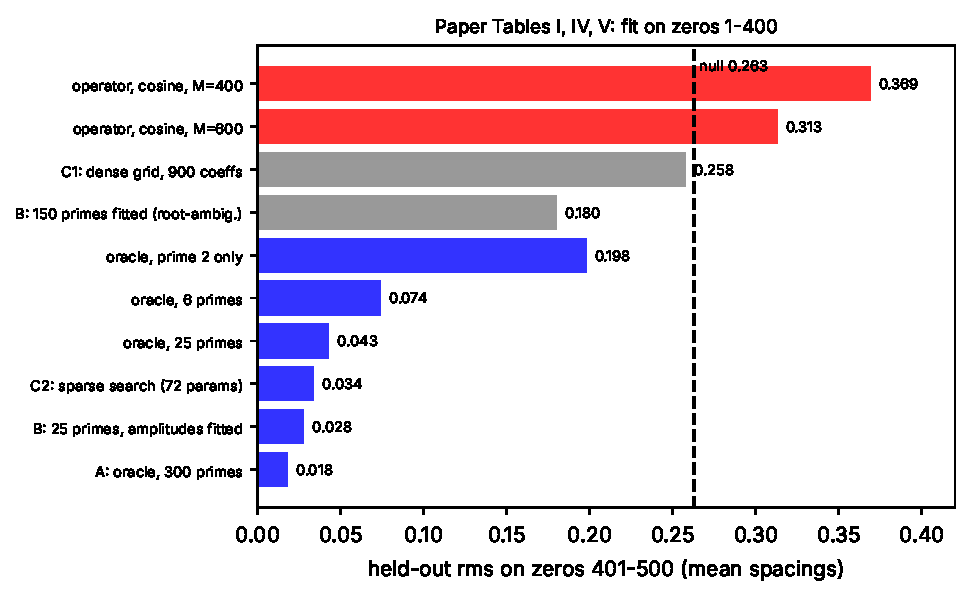
\includegraphics[width=0.85\linewidth]{figs/paper-critique_scoreboard.pdf}
\caption{Scoreboard of held-out rms errors on zeros 401--500, fit on zeros 1--400, in units of local mean spacing, as reported in paper Tables~I, IV and V. Red: fitted potentials (cosine basis). Gray: the dense Fourier control C1 (no arithmetic input, no sparsity prior) and the root-ambiguous B row. Blue: models that use arithmetic frequencies (supplied, as in the oracle and control B, or learned, as in control C2). The dashed line is the null $0.263$. Bars to the right of the dashed line are worse than predicting no fluctuation at all.}
\label{fig:paper-critique-scoreboard}
\end{figure}

It helps to compress each rms and its null into one number. The paper does not define such a number; it reports rms and null side by side. We define, as a convenience for this chapter, the \emph{relative skill}
\begin{equation}
\mathcal{S} \;=\; 1-\frac{\text{rms of the model}}{\text{rms of the null}} .
\label{eq:paper-critique-skill}
\end{equation}
A model that predicts perfectly has $\mathcal{S}=1$; a model that does exactly as well as the null has $\mathcal{S}=0$; a model that does worse than predicting nothing has $\mathcal{S}<0$.

\begin{sample}{Relative skill of the operator and of the oracle}
On zeros 401--500 the fitted cosine potential with $M=400$ coefficients scores OOS rms $0.369$ (paper Table~I), and the six-prime oracle scores $0.074$ (Table~V). The null is $0.263$. Compute $\mathcal{S}$ for both.

Step 1: For the operator, the ratio is $0.369/0.263=1.403$.

Step 2: Hence $\mathcal{S}_{\rm op}=1-1.403=-0.403$. The fitted potential is about 40\% worse than predicting no fluctuation.

Step 3: For the oracle, the ratio is $0.074/0.263=0.281$.

Step 4: Hence $\mathcal{S}_{\rm or}=1-0.281=0.719$.

$\boxed{\mathcal{S}_{\rm op}\approx-0.40,\qquad \mathcal{S}_{\rm or}\approx+0.72}$
\end{sample}

\emph{Strength and limits.} The scope sentence is the most important hedge in the paper, and it is faithful to the experiments: only Wu--Sprung backgrounds, three bases, one optimizer family, fits to at most 1000 zeros. You should carry this scope into every sentence you write about the paper.

\subsection{Paragraph 2: why the fits fail (a heuristic)}

The second paragraph begins ``The failure is intelligible, though heuristically so.'' Notice the word \emph{heuristically}: what follows is an explanation that fits the observations, not a theorem. The argument has five links.

\begin{enumerate}
\item \emph{The bases are effectively complete for in-sample level patterns.} With enough coefficients the fitted potential can shift each training level by an essentially arbitrary amount. Evidence: in-sample rms falls below $10^{-4}$ spacings on all 500 zeros at $M=900$ (Sec.~III), and the fits reach the same in-sample accuracy on permuted and phase-randomized targets as on the true zeros (Sec.~III, ``Permutation and surrogate tests''). The coverage law of Chapter~\ref{ch:fitting} predicts when completeness sets in.
\item \emph{A family that can fit anything encodes no inductive bias toward the truth} (Chapter~\ref{ch:generalization}). If every target is fitted equally well, the quality of the fit says nothing about which target is real.
\item \emph{Held-out behavior is then set by the optimizer, not the data.} Unregularized, the fit puts large structure where only held-out levels probe the potential and does harm (paper Fig.~4, Table~III); regularized, it returns to the null and not below it.
\item \emph{The controls locate the obstacle.} It is not the parameter count: the oracle keeps improving at 900 terms, and a dense 900-coefficient Fourier model (C1) gains almost nothing. It is not that the frequencies must be supplied: the sparse search C2 finds them from 400 zeros (Table~IV).
\item \emph{A heuristic reading.} The target is, by the explicit formula, an almost-periodic function of $t$ that is sparse in frequency (Chapters~\ref{ch:fourier-series} and~\ref{ch:explicit-formula}). A potential addresses each level through its classical turning point, that is, locally in energy (Chapter~\ref{ch:wkb}). On this heuristic reading, and for the parametrizations and optimizer tested, a local-in-energy vocabulary did not produce ``keep oscillating at frequency $\log 2$ forever''.
\end{enumerate}
The paragraph closes with two careful sentences: ``This is evidence about the tested parametrizations and optimizer together, not a statement about what a potential can represent. Whether the memorization result can be derived rather than measured is an open problem.''

Link 1 can be checked by a quick estimate.

\begin{sample}{Coverage threshold at the two scales}
The coverage law (Chapter~\ref{ch:fitting}; paper Sec.~III) says that the cosine family $\cos(k\pi x/L)$, $k=0,\dots,M-1$, becomes effectively complete for joint level shifts up to energy $E$ once $M\pi/L>2\sqrt{E}$. (a) At scale 1, $L=44.883$ and the top scored level has $E\approx t_{500}=811.18$. Find the smallest $M$ satisfying the law. (b) At scale 2, $L=59.957$ and the top training level of the 1--800 fits has $E\approx s_{800}\approx1184$. Repeat.

Step 1: Rearrange the inequality. Multiply both sides of $M\pi/L>2\sqrt E$ by $L/\pi$, which is positive:
\[
M>\frac{2\sqrt{E}\,L}{\pi}.
\]

Step 2: Scale 1. $\sqrt{811.18}=28.481$, so $2\sqrt E=56.963$. Multiply by $L$: $56.963\times44.883=2556.7$. Divide by $\pi$: $813.8$.

Step 3: Scale 2. $\sqrt{1184}=34.41$, so $2\sqrt E=68.81$. Multiply by $L=59.957$: $4126$. Divide by $\pi$: $1313$.

$\boxed{M_{\rm scale\,1}\gtrsim 814,\qquad M_{\rm scale\,2}\gtrsim 1313}$

Interpretation: at scale 1 the paper's statement that all 500 zeros are reproduced to rms $<10^{-4}$ ``by $M=900$'' sits just above the threshold, as the law predicts. At scale 2 the largest basis used, $M=900$, is below the threshold for the top training levels. Turning the law around, $M=900$ at scale 2 covers energies only up to
\[
E=\Bigl(\frac{M\pi}{2L}\Bigr)^2=\Bigl(\frac{900\pi}{119.914}\Bigr)^2=(23.58)^2\approx556,
\]
which is roughly the height of level 310 (because $\Nsm(556)+\tfrac12\approx310$). Levels above about 310 are not covered. This fits the observation that the in-sample rms there is still $0.103$ (Table~I). The coverage law is itself heuristic (Chapter~\ref{ch:fitting}), so these thresholds are estimates, not sharp lines.
\end{sample}

Link 3 involves a second fact worth making quantitative: a prediction that is uncorrelated with the truth cannot beat the null, however you rescale it.

\begin{sample}{What a correlation is worth}
Let $f_j$ be the true fluctuations and $g_j$ the predicted fluctuations on $n_{\rm out}$ held-out levels, $j=1,\dots,n_{\rm out}$, and suppose both have mean close to zero (true to good approximation for the zeros). Find the smallest rms you could reach by multiplying the prediction by the best constant $a$, and evaluate it for the six-prime oracle (corr $+0.96$) and the $M=400$ operator (corr $-0.07$), with null $0.263$.

Step 1: The mean squared error of the rescaled prediction is
\[
Q(a)=\frac{1}{n_{\rm out}}\sum_j (f_j-a g_j)^2 .
\]

Step 2: Differentiate with respect to $a$ and set to zero:
\[
\frac{dQ}{da}=-\frac{2}{n_{\rm out}}\sum_j g_j(f_j-a g_j)=0
\quad\Longrightarrow\quad a=\frac{\sum_j f_j g_j}{\sum_j g_j^2}.
\]

Step 3: Expand $Q$ and substitute this $a$:
\[
Q_{\min}=\frac{1}{n_{\rm out}}\Bigl[\sum_j f_j^2-2a\sum_j f_jg_j+a^2\sum_j g_j^2\Bigr]
=\frac{1}{n_{\rm out}}\Bigl[\sum_j f_j^2-\frac{(\sum_j f_jg_j)^2}{\sum_j g_j^2}\Bigr].
\]

Step 4: Factor out $\sum_j f_j^2/n_{\rm out}$, which is the square of the null rms:
\[
Q_{\min}=\text{(null rms)}^2\Bigl[1-\frac{(\sum_j f_jg_j)^2}{\sum_j f_j^2\sum_j g_j^2}\Bigr]
=\text{(null rms)}^2\,(1-r^2),
\]
where, for mean-zero sequences, $r$ is the Pearson correlation (Chapter~\ref{ch:probability}).

Step 5: Take the square root: smallest rms $=\text{null}\times\sqrt{1-r^2}$.

Step 6: Oracle: $\sqrt{1-0.96^2}=\sqrt{0.0784}=0.280$, so $0.263\times0.280=0.0736$. Operator: $\sqrt{1-0.07^2}=0.9975$, so $0.263\times0.9975=0.2624$.

$\boxed{\text{oracle: }0.074\text{ at best rescaling},\qquad\text{operator: }0.262}$

The oracle's actual rms, $0.074$ (Table~V), is consistent with its best-rescaled value within the rounding of $r$. As $r$ runs from $0.965$ down to $0.955$, the best-rescaled rms $0.263\sqrt{1-r^2}$ runs from $0.069$ up to $0.078$, so with two-digit inputs we can say only that its amplitudes are close to right. The mean-zero assumption of the sample is reasonable here: the mean of the true fluctuations on 401--500 is less than a fifth of their rms (check it with \texttt{qmnt.fluct}). The operator, even with the best possible rescaling, could only tie the null; its actual rms $0.369$ is worse because it emits uncorrelated structure of nonzero size.
\end{sample}

The statements in paragraph 2 and elsewhere in Sec.~VI have different status. \Cref{tab:paper-critique-status} sorts them, using the status labels of this book.

\begin{table}[htbp]\centering\small
\caption{Status of the main statements of the paper's Sec.~VI.}
\label{tab:paper-critique-status}
\begin{tabular}{p{6.3cm}p{3.2cm}p{3.0cm}}
\toprule
Statement & Status & Evidence in paper \\
\midrule
In-sample success coexisted with no reproducible held-out content, in the families examined & numerical observation & Tables I--III, Figs.~1, 3, 4 \\
A zero-parameter arithmetic formula carries abundant transferable content & numerical observation & Table V, Fig.~1 \\
A sparse sinusoidal fit learns that content from the same zeros & numerical observation; frequency alignment check exploratory & Table IV, Sec.~IV \\
The bases are effectively complete in-sample & numerical observation plus heuristic coverage law & Sec.~III \\
A family that fits anything has no inductive bias & general principle (heuristic) & Sec.~VI \\
Almost-periodic target versus local-in-energy parametrization & heuristic explanation & Sec.~VI, continuation probe \\
The memorization result can be derived & open problem & Sec.~VI \\
Riemann hypothesis; Hilbert--P\'olya conjecture & open; not addressed & Sec.~I \\
\bottomrule
\end{tabular}
\end{table}

\subsection{Paragraphs 3 to 5}

Paragraph 3 states the limits of the evidence; we read it in \cref{sec:paper-critique-limits}. Paragraph 4 states the broader lesson: ``Spectral agreement obtained by fitting an operator to a finite sequence establishes representational capacity, not that the fitted operator contains the mechanism generating the sequence.'' It quotes the decisive pair of intervals: principal $M=400$ held-out correlation $[-0.21,+0.08]$ against the oracle's $[+0.95,+0.97]$ on the same holdout (bootstrap intervals, Chapter~\ref{ch:controls}). Paragraph 5 proposes the falsifiability standard (read in \cref{sec:paper-critique-standard}) and closes by concluding that ``at the scales accessible to direct numerics, and within the operator families tested here, the predictable structure in the Riemann zeros is arithmetic: fully accessible, learnable from the zeros by a frequency-sparse model, and entirely missed by the inverse-spectral fits tested.'' Keep both qualifiers (scales, families) whenever you repeat this sentence.

\begin{checkpoint}
Does the paper show that no Hermitian operator can have the Riemann zeros as its spectrum?
\end{checkpoint}
\checkanswer{No. It shows that, in three bases on one background with one fitting protocol, potentials fitted to at most 1000 zeros showed no reproducible held-out skill. It says explicitly that this is ``not a statement about what a potential can represent'' and that it does not touch analytic constructions. The Hilbert--P\'olya conjecture remains open.}

\begin{keyideas}
\item Sec.~VI makes scoped numerical observations (fits memorize; arithmetic predicts; a sparse model learns), a heuristic explanation, a methodological proposal, and one open problem.
\item Relative skill \eqref{eq:paper-critique-skill} compresses rms and null into one number; the fitted operators have $\mathcal{S}<0$ on zeros 401--500.
\item A prediction uncorrelated with the truth cannot beat the null even after optimal rescaling: the best rms is null$\times\sqrt{1-r^2}$.
\item The coverage threshold $M>2\sqrt E L/\pi$ is about 814 at scale 1 and about 1313 at scale 2.
\end{keyideas}

%======================================================================
\section{The proposed falsifiability standard}\label{sec:paper-critique-standard}

A claim is \emph{falsifiable} when some possible outcome of an experiment would show it to be wrong. ``This fitted potential reproduces the first 400 zeros'' is true but almost unfalsifiable once the basis is large: Sec.~III shows the same fit reproduces shuffled zeros just as well, so no in-sample outcome could have told against it. The paper therefore proposes (Sec.~VI, paragraph 5) that any future claim that a constructed or learned operator ``captures'' the zeros be accompanied by four pieces of evidence. \Cref{fig:paper-critique-checklist} shows them as a checklist.

\begin{figure}[htbp]\centering
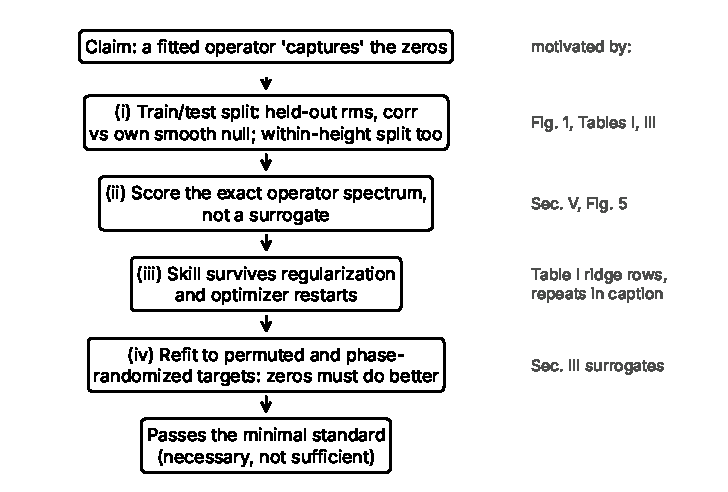
\includegraphics[width=0.85\linewidth]{figs/paper-critique_checklist.pdf}
\caption{The four-item falsifiability standard proposed in Sec.~VI of the paper, drawn as a checklist. Left: the item. Right: the experiment in the paper that shows why the item is needed. Passing all four is a minimal (necessary) condition for a ``captures the zeros'' claim, not a sufficient one.}
\label{fig:paper-critique-checklist}
\end{figure}

\subsection{Item (i): a train/test split, against the model's own null, including a within-height split}

\emph{What it says.} Fit on some zeros, predict others, report held-out rms and corr, and compare with the null of the model's own smooth part (for a fitted potential, the unperturbed background). Include at least one split in which training and held-out zeros come from the same height range.

\emph{Why ``its own null''.} Any model built on a smooth background already predicts the mean positions of the zeros. Only the fluctuations are informative. A model must be compared with the version of itself that predicts no fluctuation.

\emph{Why a within-height split.} A forward split (train low, test high) mixes two effects: failure to capture structure, and \emph{covariate shift} (Chapter~\ref{ch:generalization}), because the fluctuation amplitude grows with height (the null rises from $0.263$ on 401--500 to $0.296$ on 5001--10000, Table~V). Random 80/20 and odd/even splits inside one height range (Table~III) remove the shift. The paper's finding that the failure is even worse within height (for the random 80/20 splits, held-out errors $1.5$--$3.0$ times the null at scale 1 and $1.8$--$1.9$ times at scale 2) is what rules out covariate shift as the explanation.

\subsection{Item (ii): score the actual operator spectrum}

\emph{What it says.} If the fit used an approximation of the spectrum (a surrogate such as second-order perturbation theory), the final score must use the exact eigenvalues of the fitted operator.

Recall from Chapter~\ref{ch:non-hermitian} that Sec.~V of the paper perturbs $H\to H+iA$, with $A=\sum_k c_k\phi_k$ a real multiplication operator, in two classes. The \emph{PT-odd} class uses odd basis functions $\phi_k=\sin((k+1)\pi x/L)$. The \emph{absorptive-even} class uses even basis functions $\phi_k=\cos(k\pi x/L)$ and models a decay width $\Gamma$ through $-i\Gamma/2$. In the even class the constant function $\phi_0=1$, with coefficient $c_0$, is the \emph{null mode}: a constant $iA$ shifts every level by the same imaginary constant and has zero second-order real shift. Before it was repaired, the optimizer drove $c_0$ to about $2.2\times10^6$ by exploiting float32 noise in tensor entries that are analytically zero (Chapter~\ref{ch:paper-spurious-floor}).

\begin{sample}{Why item (ii) matters: the spurious floor in numbers}
In Sec.~V the second-order surrogate of the PT-odd fit reaches in-sample rms $0.2321$, and the absorptive-even fit (null mode repaired) reaches $0.2358$, against a null of $0.2438$. Exact diagonalization of the same fitted operators gives in-sample rms $0.2523$ and $0.2477$. Express each as a percentage improvement over the null, defined as $(\text{null}-\text{rms})/\text{null}$, so that a positive value means better than the null and a negative value means worse.

Step 1: PT-odd, surrogate: $(0.2438-0.2321)/0.2438=0.0117/0.2438=0.0480$, an apparent improvement of $4.80\%$.

Step 2: PT-odd, exact: $(0.2438-0.2523)/0.2438=-0.0085/0.2438=-0.0349$, an improvement of $-3.49\%$, i.e. $3.49\%$ \emph{worse} than the null.

Step 3: Absorptive-even, surrogate: $(0.2438-0.2358)/0.2438=0.0080/0.2438=0.0328$, an apparent improvement of $3.28\%$.

Step 4: Absorptive-even, exact: $(0.2438-0.2477)/0.2438=-0.0039/0.2438=-0.0160$, an improvement of $-1.60\%$, i.e. $1.60\%$ worse.

$\boxed{\text{improvement over null: surrogate }+4.80\%,\,+3.28\%;\qquad \text{exact }-3.49\%,\,-1.60\%}$

The sign flips. A paper that stopped at the surrogate would have reported an improvement that no operator possesses (Chapter~\ref{ch:paper-spurious-floor}).
\end{sample}

\subsection{Item (iii): survival under regularization and restarts}

\emph{What it says.} A claimed skill should persist when the fit is mildly regularized (ridge, Chapter~\ref{ch:least-squares}) and when the optimizer is started from different random initial coefficients.

\emph{Why.} A skill that appears for one starting point only, or that vanishes under a mild ridge, is a property of the optimizer's path, not of the data. In the paper, the ridge rows of Table~I ($\mu=0.03$, $0.3$) and the random-init repeats in the Table~I caption (OOS $0.365$--$0.379$ over four repeats) show that the negative result is stable. For the interpolation split, ridge ``removes the damage and nothing else'' (Sec.~III).

\begin{pitfall}
Item (iii) is phrased for \emph{positive} claims. When a ridge returns a fit to the null (as in Tables~I and II), that does not make the fit predictive; it makes it inert. ``Survives regularization'' means that the skill survives, not that the error stops being worse than the null.
\end{pitfall}

\subsection{Item (iv): refit to permuted and phase-randomized targets}

\emph{What it says.} Repeat the whole fit on surrogate targets: the true fluctuation sequence randomly permuted (marginal distribution kept, order destroyed) and phase-randomized~\cite{theiler} (power spectrum kept, phases scrambled), as in Chapter~\ref{ch:controls}.

\emph{Why.} If the model fits surrogates as well as the zeros, in-sample accuracy measures capacity. Sec.~III reports in-sample rms $0.134\pm0.010$ (permuted), $0.141\pm0.006$ (phase-randomized) and $0.138\pm0.005$ (amplitude-adjusted~\cite{schreiber}), against $0.137$ on the true zeros. The zeros are not special to the fit.

\subsection{What the standard does and does not guarantee}

The paper calls held-out prediction a ``minimal'' standard. Two consequences follow.

\emph{It is necessary, not sufficient.} Passing all four items does not show that a model is ``the'' zeta operator. The simple kriging interpolator of Sec.~III predicts held-out zeros within one height range at rms $0.117$, correlation $+0.87$, and the sparse sinusoidal model C2 predicts at $+0.99$; neither is an operator at all. Passing the standard shows that a model has captured \emph{some} transferable structure.

\emph{It does not apply to analytic constructions in the same way.} If an operator is specified without looking at any zero (for example, constructions built only from primes~\cite{connes26,zetatriples}), every zero is held out. The paper notes that for such constructions ``no held-out evaluation question arises''; they are judged by direct comparison with all zeros.

\begin{checkpoint}
A hypothetical paper fits a 500-coefficient potential to zeros 1--400 and reports in-sample rms $10^{-5}$, held-out rms $0.262$ on 401--500 (null $0.263$), and held-out corr $+0.02$. Which items of the standard has it addressed, and does it support a ``captures'' claim?
\end{checkpoint}
\checkanswer{It has addressed half of item (i): a forward split with rms and corr against the null, but no within-height split. Items (ii)--(iv) are not reported. In any case the numbers show no skill: $\mathcal S=1-0.262/0.263\approx0.004$ and a correlation of $+0.02$, which is indistinguishable from zero for 100 levels (for 100 independent pairs, the standard error of a correlation near zero is about $1/\sqrt{100}=0.1$). The claim is not supported.}

\begin{checkpoint}
Why must item (ii) be checked separately from item (i)? Could a model pass (i) using surrogate spectra and fail (ii)?
\end{checkpoint}
\checkanswer{Yes. Item (i) can be computed with whatever spectrum the fit used. If that spectrum is an approximation (such as the second-order formula, paper Eq.~(5)) and the fitted amplitudes are outside its range of validity, the approximate held-out scores need not describe the actual operator. Sec.~V shows exactly this for in-sample scores: surrogate $0.2321$, exact $0.2523$.}

\begin{keyideas}
\item The standard: (i) held-out rms and corr against the model's own null, including a within-height split; (ii) exact spectra; (iii) robustness to ridge and restarts; (iv) surrogate refits.
\item Each item is motivated by a specific experiment in the paper (Tables~I and III; Sec.~V; Table~I ridge rows and repeats; Sec.~III surrogates).
\item The standard is a minimal necessary condition; non-operator models such as kriging and C2 also pass item (i).
\end{keyideas}

%======================================================================
\section{The limits the paper states}\label{sec:paper-critique-limits}

Paragraph 3 of Sec.~VI states five limits. A good habit is to ask of each: \emph{what would change if this limit were removed, and in which direction?}

\subsection{Limit 1: one background, three bases}

``One background potential (Wu--Sprung) and three bases were tested; Hermite, wavelet, and neural-network parametrizations were not''. The hat basis is described as ``the simplest stand-in for a wavelet-type basis'' (Sec.~II~C), not as a wavelet basis. The direction of the uncertainty is one-sided: an untested basis could in principle show skill; nothing tested so far gives reproducible evidence that it would (one Chebyshev row is marginal; see Limit 2). We return to this in \cref{sec:paper-critique-weak} (W2).

\subsection{Limit 2: one marginal Chebyshev row}

Table~II has eight rows. One, Chebyshev $M=400$, has OOS rms $0.291$ (interval $[0.25,0.33]$, which contains the null $0.263$) and corr $+0.18$ with interval $[-0.02,+0.37]$, whose lower end is at zero. The paper says ``one such row among eight is not evidence of prediction, but a small positive correlation for this row is not excluded.'' How surprised should we be by one such row?

\begin{sample}{One marginal row among eight}
Suppose (heuristically) that every row in Table~II had true correlation zero, and that for each row independently the chance that its 95\% percentile interval lies entirely at or above zero is $\alpha=0.025$ (one tail of a 95\% interval). What is the probability that at least one of the $k=8$ rows looks like the Chebyshev row or better? What is the expected number of such rows?

Step 1: The probability that a given row does \emph{not} show this is $1-\alpha=0.975$.

Step 2: By independence (Chapter~\ref{ch:probability}), the probability that none of the $k$ rows shows it is the product of the individual probabilities:
\begin{equation}
P(\text{none})=(1-\alpha)^k .
\label{eq:paper-critique-none}
\end{equation}

Step 3: ``At least one'' is the complement:
\begin{equation}
P(\text{at least one})=1-(1-\alpha)^k .
\label{eq:paper-critique-atleastone}
\end{equation}

Step 4: Numerically, $0.975^8=0.8167$, so $P=1-0.8167=0.183$.

Step 5: The expected number is $k\alpha=8\times0.025=0.2$.

$\boxed{P(\text{at least one})\approx0.18,\qquad \text{expected count}=0.2}$

So roughly one time in five a table of eight null rows would contain one row this good. The assumptions are rough: rows share the same training and held-out zeros, so they are not independent; bootstrap intervals are approximate; and the Chebyshev interval's lower end is ``at zero'', not above it. The calculation supports the paper's wording, neither stronger nor weaker: not evidence of prediction, not excluded.
\end{sample}

Table~II also contains one row whose correlation interval lies entirely \emph{below} zero: hat, $M=400$, $[-0.37,-0.01]$. Count excursions of either sign. A 95\% interval of a null row then excludes zero with probability $\alpha=0.05$, and \eqref{eq:paper-critique-atleastone} gives $1-0.95^8\approx0.34$ for at least one such row among eight. Excursions of either sign are what a table of null rows produces, and one positive and one negative excursion among eight rows fit that picture.

\subsection{Limit 3: heights}

``The operator fits use at most the first 1000 zeros, and the fitted sinusoidal controls were scored only below zero 2000.'' The oracle, which has no fitted parameters, was scored through zero $10^4$ (Table~V).

Why does height matter for the fitted controls? Because estimated frequencies dephase. The paper reports that C2's skill falls from $0.034$/$+0.99$ on 401--500 to $0.078$/$+0.96$ on zeros 1001--2000 (Sec.~IV). Chapter~\ref{ch:sparse-frequency} explained the mechanism; here is the worst-case size.

\begin{sample}{Worst-case dephasing beyond the training window}
Control C2 fitted on zeros 1--400 scores $0.034$/$+0.99$ on 401--500 and $0.078$/$+0.96$ on 1001--2000 (Sec.~IV). To see why skill must eventually decay, suppose a model learns the $p=2$ frequency $\omega=\log 2$ from the window of zeros 1--400, of length $T=t_{400}-t_1$ in $t$, with an error $\delta\omega$ no larger than half a Fourier resolution cell, $\abs{\delta\omega}\le\pi/T$. This bound is the tolerance the paper uses when matching selected frequencies to prime powers (App.~A step 23). It is an upper bound, not a measured error, and Step 6 shows that a good fit cannot come close to it. Assume the learned and true waves agree in phase at the end of the window, $t_*=t_{400}$. Find the phase error of the fundamental $m=1$ at $t_{1001}$ and at $t_{2000}$, the two ends of the paper's 1001--2000 holdout.

Step 1: The true phase of the $m$-th harmonic is $m\omega t+\varphi$, the learned phase is $m(\omega+\delta\omega)t+\hat\varphi$. Agreement at $t_*$ fixes $\hat\varphi=\varphi-m\,\delta\omega\,t_*$.

Step 2: Subtract the two phases at a general $t$:
\begin{equation}
\delta\phi_m(t)=m(\omega+\delta\omega)t+\varphi-m\,\delta\omega\,t_*-(m\omega t+\varphi)=m\,\delta\omega\,(t-t_*).
\label{eq:paper-critique-dephase}
\end{equation}

Step 3: Window: $T=t_{400}-t_1\approx666$ (computed with \texttt{qmnt.zeros}), so the largest allowed frequency error is $\pi/T\approx0.00472$.

Step 4: Distances, from \texttt{qmnt.zeros(2000)}: $t_{1001}-t_{400}\approx741$ and $t_{2000}-t_{400}\approx1836$.

Step 5: By \eqref{eq:paper-critique-dephase} with $m=1$: $\delta\phi_1\approx0.00472\times741\approx3.5$ rad at $t_{1001}$, and $\delta\phi_1\approx0.00472\times1836\approx8.7$ rad at $t_{2000}$. The third harmonic, $m=3$, has three times these phase errors.

$\boxed{\delta\phi_1\approx3.5\text{ rad at }t_{1001},\qquad \delta\phi_1\approx8.7\text{ rad at }t_{2000}}$

Step 6: Why the bound is far from a typical error. Apply \eqref{eq:paper-critique-dephase} inside the window. Between $t_1$ and $t_{400}$ an error $\delta\omega=\pi/T$ produces a phase drift $\delta\omega\,T=\pi$, half a cycle. A learned wave that slides half a cycle out of step across its own training data cannot fit those data well. So a model that does fit them must have $\abs{\delta\omega}$ well below $\pi/T$. Chapter~\ref{ch:sparse-frequency} showed that the least-squares frequency error scales like $1/T$ times a factor that shrinks as the number of samples and the signal-to-noise ratio grow. If, for illustration, $\abs{\delta\omega}$ were a tenth of the bound, the fundamental's phase error at $t_{2000}$ would be about $0.87$ rad. (We matched the phase at the end of the window for simplicity. A least-squares fit tends to get the phase right nearer the middle of the window. That would add $\delta\omega\,T/2$ to every phase error beyond the window, so matching at the end understates the error rather than exaggerating it.)

What the sample shows is the shape, not the size. The phase error grows linearly with distance from the window, so any learned frequency model has a finite range of validity in height (C2's rms rises from $0.034$ on 401--500 to $0.078$ on 1001--2000). The exact frequencies $m\log p$ of the oracle never dephase (Table~V).
\end{sample}

\Cref{fig:paper-critique-dephase} draws this worst case for the prime-2 wave of running example RE2.

\begin{figure}[htbp]\centering
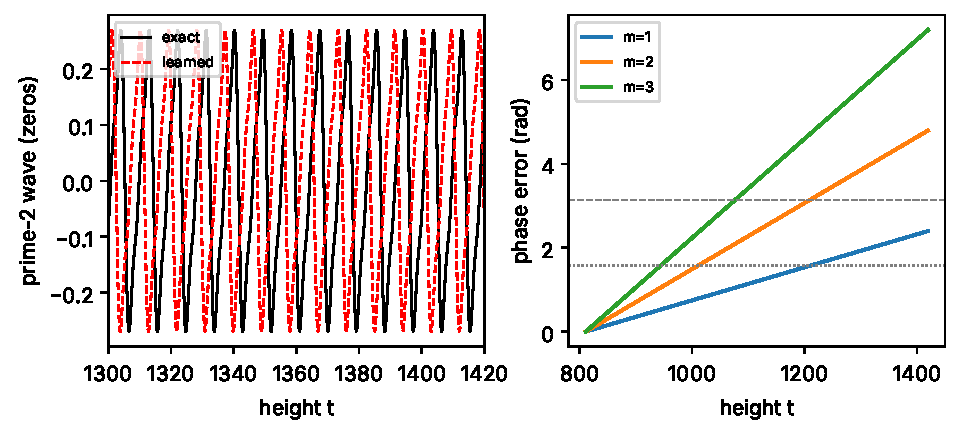
\includegraphics[width=0.85\linewidth]{figs/paper-critique_dephase.pdf}
\caption{Worst-case dephasing of the prime-2 wave (RE2), $-\frac1\pi\sum_{m=1}^{3}\sin(mt\omega)/(m2^{m/2})$. The frequency is learned from zeros 1--400. Left: near $t_{1001}$, the exact wave ($\omega=\log2$, solid) and a learned wave whose frequency is off by the matching tolerance $\delta\omega=\pi/T$, with $T=t_{400}-t_1$ (dashed). The two waves are matched in phase at $t_{400}$, and the vertical line marks $t_{1001}$. Right: magnitude of the phase error, $m\,\delta\omega\,\abs{t-t_{400}}$, in radians for $m=1,2,3$, with $\pi/2$ and $\pi$ marked and vertical lines at $t_{400}$, $t_{1001}$ and $t_{2000}$. The horizontal axes are the height $t$. The tolerance is an upper bound, much larger than the error of a good fit (see text).}
\label{fig:paper-critique-dephase}
\end{figure}

\subsection{Limit 4: Sec.~V was not rerun}

``The non-Hermitian analysis of Sec.~V is inherited from the original computation and was not rerun for this revision.'' Sec.~V's numbers (the floors, the null-mode artifact with $c_0\approx2.2\times10^6$, the exact-versus-surrogate comparison) therefore rest on the original computation. The paper also states that the Hermitian conclusions of Secs.~III and IV ``do not depend on'' Sec.~V. We give a cheap partial check in \cref{sec:paper-critique-weak} (W4).

\subsection{Limit 5: bootstrap independence}

``Bootstrap intervals resample held-out levels independently except where stated.'' Independent resampling can misestimate uncertainty when neighboring values are correlated (Chapter~\ref{ch:controls}). Consider the mean of $n$ values with standard deviation $\sigma$. Its variance is $\sigma^2/n$ plus $2/n^2$ times the sum of the covariances of all pairs. That variance equals $\sigma^2/n$ only when those covariances vanish. Positive correlations between neighbors increase it and negative correlations decrease it. Independent resampling ignores these pair terms, so it understates the uncertainty in the first case and can overstate it in the second. The zeros' fluctuations have negative autocorrelation at lags 1--3 (Sec.~III), and for statistics such as rms and corr the direction of the effect is not obvious in advance. The paper reran the Table~II intervals with a moving-block bootstrap (block lengths 3 to 20) and reports that ``they widen slightly and no conclusion changes (for the cosine row, at most $[0.30,0.44]$).'' You can see the effect yourself on the six-prime oracle in \cref{fig:paper-critique-block}.

\begin{figure}[htbp]\centering
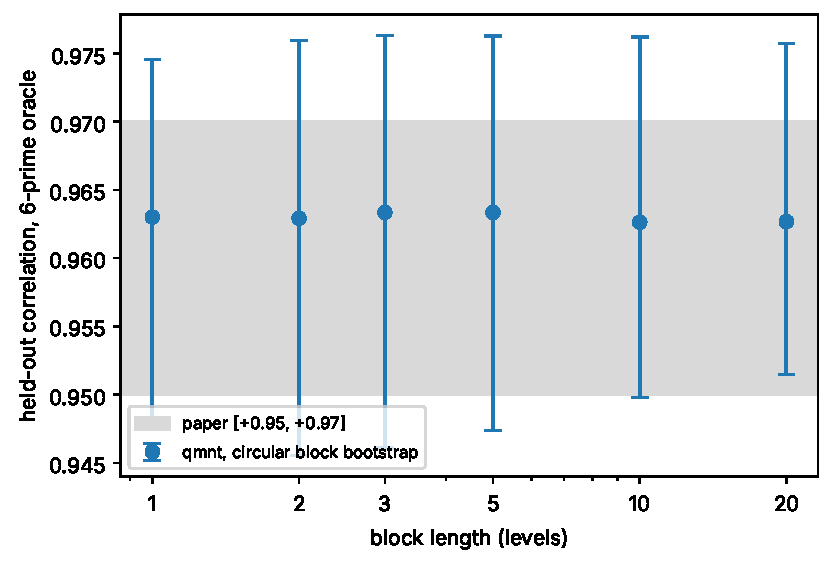
\includegraphics[width=0.85\linewidth]{figs/paper-critique_block.pdf}
\caption{Percentile 95\% bootstrap intervals for the held-out correlation of the six-prime oracle on zeros 401--500, computed with \texttt{qmnt} by circular block bootstrap, as a function of block length (block length 1 is independent resampling, as in most of the paper's intervals). The gray band is the paper's reported interval $[+0.95,+0.97]$ (Sec.~III and Table~V caption). Compare the widths at different block lengths to see how serial correlation affects the interval.}
\label{fig:paper-critique-block}
\end{figure}

\begin{checkpoint}
Limit 5 concerns intervals, not point estimates. Could switching to a block bootstrap ever turn the operator's OOS rms $0.369$ into a value below the null?
\end{checkpoint}
\checkanswer{No. The bootstrap changes the interval around an estimate, not the estimate. The point value $0.369$ is computed once from the held-out levels. A wider interval could at most make the comparison with the null less decisive; the paper reports that even with blocks the cosine row's interval is at most $[0.30,0.44]$, still above $0.263$.}

\begin{keyideas}
\item The paper's stated limits: one background and three bases; one marginal Chebyshev row; operator fits to at most zero 1000 and fitted controls scored below zero 2000; Sec.~V not rerun; mostly independent bootstrap.
\item One marginal row among eight is expected about one time in five under rough independence, \eqref{eq:paper-critique-atleastone}.
\item A learned frequency dephases linearly with distance, \eqref{eq:paper-critique-dephase}; with the matching tolerance as the worst case, a frequency learned from zeros 1--400 could be about 3.5 rad out of phase at $t_{1001}$. A good fit does much better, but the linear growth with distance is unavoidable.
\end{keyideas}

%======================================================================
\section{Weak points a referee could press}\label{sec:paper-critique-weak}

A referee's job is to find the places where a paper's conclusions are least secure. Below are the points a well-informed skeptic could raise. Several overlap with the stated limits; others are not listed in Sec.~VI. For each we say what the paper itself says, how much weight the point carries, and what would resolve it. Raising a point is not the same as refuting a claim.

\subsection{W1: the literature-gap claim rests on a keyword audit}

Sec.~I~A states: ``to our knowledge, no systematic held-out test of predictive performance has been reported in this literature''. The basis (App.~A, ``Literature audit'') is: among all works citing Wu--Sprung~\cite{wusprung} and van Zyl--Hutchinson~\cite{vanzyl} indexed by Semantic Scholar (accessed August 2026; 28 and 29 works respectively; Slater~\cite{slater} and Jaksch~\cite{jaksch} had no indexed citations), none mentions prediction, generalization, held-out evaluation, or machine learning.

A referee could press three points. (a) Coverage: a database does not index everything, and relevant work need not cite these two papers. (b) Keywords: a held-out test might be described as ``extrapolation'' or ``testing on higher zeros''. (c) Sample size: a few dozen works is a small sample. The paper hedges with ``to our knowledge'' and records the audit so that it can be checked. How strong is ``none of $n$''?

\begin{sample}{What ``none out of $n$'' can support}
Treat each citing work, heuristically, as an independent draw that reports a held-out test with unknown probability $f$. If none of $n$ works does, find the value $f_{95}$ above which observing ``none'' would have probability below 5\%. Evaluate for $n=29$ (if the two citing sets overlap completely, the distinct works number at least 29) and $n=57=28+29$ (no overlap).

Step 1: For one work, the probability of no held-out test is $1-f$. For $n$ independent works, $P(\text{none})=(1-f)^n$, the same reasoning as \eqref{eq:paper-critique-none}. The independence assumption is rough: the 28 and 29 citing works overlap, may cite one another, and are not random draws from the literature, so what follows is an order-of-magnitude guide, not a precise bound.

Step 2: Set $(1-f_{95})^n=0.05$ and take the $n$-th root: $1-f_{95}=0.05^{1/n}$, so
\begin{equation}
f_{95}=1-0.05^{1/n}.
\label{eq:paper-critique-rule3}
\end{equation}

Step 3: Approximate for large $n$. Write $0.05^{1/n}=e^{(\log 0.05)/n}$ and use $\log0.05=-2.996\approx-3$ and $e^{-y}\approx1-y$ for small $y$ (Chapter~\ref{ch:asymptotics}): $f_{95}\approx 3/n$, the ``rule of three''.

Step 4: $n=29$: $(\log0.05)/29=-0.10330$, $e^{-0.10330}=0.90186$, so $f_{95}=0.0981$ (rule of three: $3/29=0.103$).

Step 5: $n=57$: $(\log0.05)/57=-0.05256$, $e^{-0.05256}=0.94880$, so $f_{95}=0.0512$ (rule of three: $3/57=0.053$).

$\boxed{f_{95}\approx0.098\ (n=29),\qquad f_{95}\approx0.051\ (n=57)}$

Interpretation: the audit supports ``held-out tests are rare in this citation neighborhood (probably under one work in ten, and under about one in twenty if the two citing lists do not overlap)'' more firmly than ``there are none anywhere''. Keyword misses (point b) would make $f_{95}$ larger still (Problem 25). The paper's own wording, ``to our knowledge'', is the appropriate strength.
\end{sample}

\subsection{W2: one background potential}

Every fitted potential is a correction $\delta V$ added to the Wu--Sprung potential (Chapter~\ref{ch:wu-sprung}). The background fixes which part of space each level probes, through the classical turning point $x_E$ with $V(x_E)=E$ (Chapter~\ref{ch:wkb}). A referee could ask whether a different background (one with fluctuation structure already built in, such as Wu and Sprung's own fractal corrections, or a different confining shape) would change the conclusion. The paper does not test this and says so.

The turning-point map is easy to compute and makes the question concrete.

\begin{sample}{Turning points of the interpolation gap}
The paper states that ``levels 201--300 turn at $x=22.5$--$28.5$'' (Sec.~III, interpolation split). Check this with \texttt{qmnt}, using the smooth zeros $s_{201}$ and $s_{300}$ as the level energies and the Wu--Sprung relation $x(V)$ of paper Eq.~(2).

Step 1: For an even, monotone potential, a level of energy $E$ turns where $V(x)=E$, so the turning point is $x(E)$, the Wu--Sprung function evaluated at $V=E$.

Step 2: Compute $s_{201}$ by solving $\Nsm(s)=200.5$ and $s_{300}$ by solving $\Nsm(s)=299.5$, with \texttt{qmnt.smooth\_zeros} (the listing after this sample). This gives $s_{201}\approx398$ and $s_{300}\approx543$.

Step 3: Evaluate Eq.~(2) at these energies (with \texttt{qmnt.wu\_sprung\_x}, in the same listing): $x(s_{201})\approx22.5$ and $x(s_{300})\approx28.5$.

$\boxed{x\approx22.5\ \text{to}\ 28.5}$

This agrees with the paper. With a different background $V$, the same levels would turn at different places, and the region where an unregularized fit can ``do damage at no in-sample cost'' (paper Fig.~4) would move.
\end{sample}

\begin{pycode}
import numpy as np, qmnt
s = qmnt.smooth_zeros(np.array([201, 300]))   # energies of levels 201 and 300
x = qmnt.wu_sprung_x(s)                       # turning points, paper Eq. (2)
print(s, x)                                   # about [398, 543] and [22.5, 28.5]
\end{pycode}

\begin{figure}[htbp]\centering
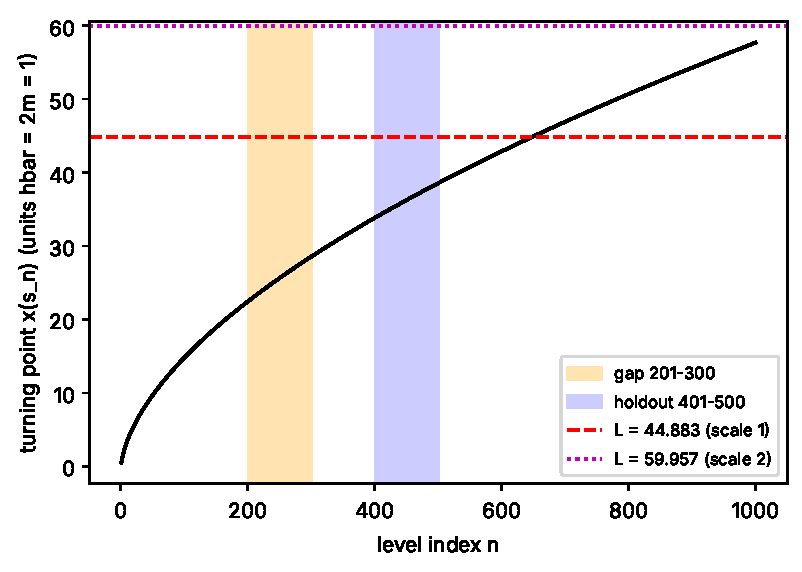
\includegraphics[width=0.85\linewidth]{figs/paper-critique_turning.pdf}
\caption{Classical turning point $x(s_n)$ of level $n$ in the Wu--Sprung potential (paper Eq.~(2)), for $n=1$ to $1000$, in units $\hbar=2m=1$. Horizontal lines: the box half-widths $L=44.883$ (scale 1) and $L=59.957$ (scale 2). Shaded: the interpolation gap 201--300 and the principal holdout 401--500. Each held-out band of levels probes its own band of positions most strongly; the background potential fixes this map.}
\label{fig:paper-critique-turning}
\end{figure}

\subsection{W3: height range of the operator fits}

Operator fits stop at zero 1000. A referee could ask two questions: would larger fits behave differently, and how saturated are the held-out fits? Apply the coverage law of \cref{sec:paper-critique-claims} to the training ranges.

At scale 1 the principal fits train on zeros 1--400. With $E\approx s_{400}\approx680$, the threshold is $2\sqrt{680}\times44.883/\pi\approx745$. The bases used, $M=200$ to $600$, give $M/745\approx0.27$ to $0.81$.

At scale 2 the fits train on zeros 1--800. The threshold is about 1313, and $M=300$ to $900$ give $0.23$ to $0.69$.

So the held-out fits at \emph{both} scales are below the heuristic coverage threshold for their top training levels, by comparable factors. Only the in-sample coverage run on all 500 zeros at scale 1, with $M=900$ above its threshold of about 814, is fully saturated. The negative result held across this whole range of $M$ relative to the threshold: the scale-2 rows sit at or above their null $0.274$, as the scale-1 rows sit at or above theirs. Fits at higher zeros are a research project (\cref{sec:paper-critique-projects}).

\subsection{W4: Sec.~V inherited, not rerun}

The paper states this limit itself. A reader can do one cheap structural check of Sec.~V~A without rerunning anything: the sum rule $\sum_n\delta E_n=0$ is the second-order piece of an exact identity.

\begin{beyond}
\textbf{Taken on trust: trace equals the sum of eigenvalues.} For any $n\times n$ complex matrix, the sum of its eigenvalues, counted with multiplicity, equals its trace (the sum of its diagonal entries). The proof compares the coefficient of $\lambda^{n-1}$ in the characteristic polynomial $\det(\lambda I-B)$ written two ways: as $\prod_k(\lambda-\lambda_k)$ and by expanding the determinant. Recall the $2\times2$ case from Chapter~\ref{ch:eigen}, where the characteristic polynomial is $\lambda^2-(\text{trace})\lambda+\det$, so the two eigenvalues add up to the trace. For the general case see the chapter on eigenvalues and eigenvectors in \cite{strang}.
\end{beyond}

Apply it to the truncated matrix of $H+iA$ in the unperturbed eigenbasis: its diagonal entries are $E_n+iA_{nn}$, with $A_{nm}=\langle n|A|m\rangle$ real for a real multiplication operator $A$. The sum of exact eigenvalues $\lambda_n$ is therefore
\begin{equation}
\sum_n\lambda_n=\sum_n E_n+i\sum_n A_{nn}
\quad\Longrightarrow\quad
\sum_n\bigl(\Re\lambda_n-E_n\bigr)=0 .
\label{eq:paper-critique-trace}
\end{equation}
This is a statement about a finite matrix: the $\lambda_n$ here are the eigenvalues of the truncated matrix of $H+iA$ in the chosen basis of unperturbed states, not of the full operator on the whole (infinite-dimensional) space. For that finite matrix the exact real shifts sum to zero. The second-order sum rule is one piece of this identity, as the following argument shows.

Replace $A$ by $\epsilon A$, with $\epsilon$ a real bookkeeping parameter. Suppose the unperturbed levels $E_n$ are distinct, so that each eigenvalue can be expanded as a power series in $\epsilon$ (Chapter~\ref{ch:perturbation}):
\[
\lambda_n(\epsilon)=E_n+\epsilon a_n+\epsilon^2 b_n+\order(\epsilon^3).
\]
Chapter~\ref{ch:non-hermitian} found $a_n=iA_{nn}$. It also found, from second-order perturbation theory with $V\to iA$ (the product of two matrix elements carries $i^2=-1$), that
\[
b_n=-\sum_{m\ne n}\frac{A_{nm}^2}{E_n-E_m},
\]
which is the shift $\delta E_n$ of paper Eq.~(5). The trace identity holds for every $\epsilon$:
\[
\sum_n\lambda_n(\epsilon)=\sum_nE_n+i\epsilon\sum_nA_{nn}.
\]
The right side has no $\epsilon^2$ term. Two power series in $\epsilon$ that agree for all small $\epsilon$ have equal coefficients. Comparing the coefficients of $\epsilon^2$ therefore gives $\sum_n b_n=\sum_n\delta E_n=0$. The same comparison at every higher power shows that each order sums to zero separately. Our reading, which is this chapter's interpretation and not a statement in the paper, is therefore that the second-order sum rule verified in Sec.~V~A (to $3.6\times10^{-15}$ and $1.4\times10^{-14}$) checks that the code is internally consistent rather than telling us anything about the zeros. The paper itself concludes, on other grounds, that the floor is ``not a physically meaningful constant''.

A three-level example makes this concrete. Take $E=(1,2,4)$ and real symmetric $A$ with zero diagonal, $A_{12}=0.05$, $A_{13}=0.1$, $A_{23}=0.15$. Paper Eq.~(5) gives
\begin{align*}
\delta E_1&=-\Bigl[\frac{0.0025}{1-2}+\frac{0.01}{1-4}\Bigr]=-[-0.0025-0.003333]=0.005833,\\
\delta E_2&=-\Bigl[\frac{0.0025}{2-1}+\frac{0.0225}{2-4}\Bigr]=-[0.0025-0.01125]=0.00875,\\
\delta E_3&=-\Bigl[\frac{0.01}{4-1}+\frac{0.0225}{4-2}\Bigr]=-[0.003333+0.01125]=-0.014583,
\end{align*}
and the sum is $0.005833+0.00875-0.014583=0$. An exact diagonalization of the $3\times3$ matrix $\mathrm{diag}(1,2,4)+iA$ (for example with \texttt{numpy.linalg.eigvals}) gives real parts that agree with $E_n+\delta E_n$ to better than $10^{-3}$, and whose sum is exactly the trace, 7.

\subsection{W5: the frequency-alignment statistic was defined after seeing the data}

Sec.~IV reports that every frequency selected by C2 lies within half a Fourier resolution cell of some $\log q$, $q$ a prime power, and that a surrogate ensemble (900 replicates) never approaches the real zeros' alignment (App.~A step 23: cutoff-maximized binomial scores $24.7$ and $50.9$ on the real zeros, at most $4.7$ on surrogates). The paper is explicit that ``the statistic was defined after the data were seen, so the check is exploratory'' and that ``no significance claim is made here beyond the size of the ensembles.''

The paper describes the score only briefly, as a ``cutoff-maximized binomial score'' and as ``a statistic that does not depend on a chosen frequency cutoff''. Our reading, in outline, has three steps. First, count how many selected frequencies lie within $\pi/T$ of $\log q$ for some prime power $q$ up to a cutoff. Second, compare that count with a binomial distribution, which gives the number of chance matches if each frequency matched independently with a chance probability of the kind estimated in the sample below. The less probable the observed count under that model, the larger the score. Third, maximize the score over the cutoff, so that no single cutoff has to be chosen by hand. The exact definition is in the Zenodo record~\cite{zenodo}, and Chapter~\ref{ch:paper-arithmetic} discusses it. What matters here is the comparison: $24.7$ and $50.9$ on the real zeros against at most $4.7$ on any surrogate.

Why is a surrogate check needed at all? Because chance alignment is common at high frequency, where prime powers crowd together.

\begin{sample}{How often does a random frequency land near some $\log q$?}
Use the prime number theorem (Chapter~\ref{ch:primes}): near $x$, primes occur with density about $1/\log x$ per unit of $x$. Estimate the expected number $\bar m(\omega)$ of primes $q$ with $\abs{\omega-\log q}<\pi/T$, and the probability of at least one, at $\omega=2$, $5$ and $8$, for the 400-zero window $T=t_{400}-t_1\approx666$.

Step 1: The number of primes in $[x,x+\dd x]$ is about $\dd x/\log x$.

Step 2: Change variable to $\omega=\log x$: $x=e^\omega$, $\dd x=e^\omega\,\dd\omega$, $\log x=\omega$. The number of primes with $\log q$ in $[\omega,\omega+\dd\omega]$ is about $(e^\omega/\omega)\,\dd\omega$.

Step 3: The matching window has width $2\pi/T$ in $\omega$. If it is narrow compared with the scale on which $e^\omega/\omega$ changes,
\begin{equation}
\bar m(\omega)\approx\frac{2\pi}{T}\,\frac{e^\omega}{\omega}.
\label{eq:paper-critique-density}
\end{equation}
Prime powers $p^m$ with $m\ge2$ add only a few more, so we neglect them.

Step 4: Make a heuristic assumption: treat the $\log q$ near $\omega$ as if they were scattered at random and independently of one another, that is, as a Poisson process with the density of Step 3 (Chapter~\ref{ch:level-statistics}). This is a model, not a theorem. Real primes have correlations (for example, every prime above 2 is odd, so two primes above 2 are never adjacent integers), and these correlations are neglected. Under the assumption, the probability of no point in a window with expected count $\bar m$ is $e^{-\bar m}$, so $P(\ge1)=1-e^{-\bar m}$.

Step 5: $2\pi/666=0.009434$. At $\omega=2$: $e^2/2=3.695$, $\bar m=0.0349$, $P=0.034$. At $\omega=5$: $e^5/5=29.68$, $\bar m=0.280$, $P=0.244$. At $\omega=8$: $e^8/8=372.6$, $\bar m=3.52$, $P=1-e^{-3.52}=0.970$.

$\boxed{P(\text{chance match})\approx0.03\ (\omega=2),\ 0.24\ (\omega=5),\ 0.97\ (\omega=8)}$

So near the top of C2's search band ($\omega<8$, and $\log3000=8.006$) almost any frequency ``matches'' some prime power. The evidence of alignment rests on the low-frequency selections and on the collective comparison with surrogates, which is consistent with the paper's decision to check the alignment against a surrogate ensemble (its stated reason: ``the frequencies are the output of a search'') and to use a statistic that does not depend on a chosen frequency cutoff. These are heuristic estimates (density from the prime number theorem, Poisson approximation, prime powers neglected).
\end{sample}

You can count the actual prime powers in each window with the following listing and compare with \eqref{eq:paper-critique-density}.

\begin{pycode}
import numpy as np, qmnt
t = qmnt.zeros(400)
T = t[-1] - t[0]                 # length of the 400-zero window in t
q = []                           # all prime powers up to 3000
for p in qmnt.primes_upto(3000):
    pk = int(p)
    while pk <= 3000:
        q.append(pk)
        pk = pk * int(p)
logq = np.log(np.array(q, dtype=float))
for w in (2.0, 5.0, 8.0):
    count = np.sum(np.abs(logq - w) < np.pi / T)
    estimate = (2 * np.pi / T) * np.exp(w) / w
    print(w, count, round(estimate, 3))
\end{pycode}

\subsection{W6: the explanation is heuristic, and the optimizer is part of the result}

The paper says the explanation is heuristic and that the evidence is ``about the tested parametrizations and optimizer together''. A referee could press: the Hermitian fits use a specific Levenberg--Marquardt schedule (App.~A step 6) with at most 60 iterations in the revision computations; a different optimizer, or a prior on $\delta V$ that favors long-range oscillation in energy, might behave differently. The paper's within-height and interpolation results show that, under this protocol, the fit actively places structure where only held-out levels look; it does not show that no protocol could interpolate. The paper says this explicitly for the interpolation split.

\subsection{W7: the memorization result is measured, not derived}

``Whether the memorization result can be derived rather than measured is an open problem.'' A derivation would explain, for example, why held-out correlations cluster near zero rather than at some small positive value. A starting point is suggested in \cref{sec:paper-critique-projects}.

\subsection{W8: smaller points}

\begin{itemize}
\item \emph{Seed ranges are not standard errors.} Table~III's caption says so: the seeds reuse the same zeros.
\item \emph{One relaxed row.} The scale-2 $M=300$ row of Table~I used a relaxed acceptance threshold; under the strict protocol ``the optimizer accepts no step at all''. The paper labels it a sensitivity result.
\item \emph{The factor $\gtrsim1.3$.} Sec.~IV says one prime beats every fitted operator's holdout performance by a factor $\gtrsim1.3$. From the tables we can check this only for operator rows scored on the same holdout as the tabulated one-prime oracle, zeros 401--500, where the oracle scores $0.198$ (Table~V). Among those rows the lowest Table~I OOS rms is $0.265$ (ridge $\mu=0.3$), giving $0.265/0.198=1.34$; the lowest Table~II row, Chebyshev with ridge $\mu=0.3$ at $0.264$, gives $0.264/0.198=1.33$. Both clear 1.3, but only just. Table~I rows fitted on 1--300, 1--350 or 1--450, and the scale-2 rows, are scored on other holdouts, for which Table~V gives no matching one-prime entry, so this check does not cover them. Problem 6 asks you to redo the computation.
\item \emph{Two nulls.} The operator null and the smooth-zero null are conceptually distinct; the paper notes that their numerical coincidence on 401--500 (both $0.2631$) is what permits a single baseline (Sec.~II~C).
\item \emph{The oracle is not a fair competitor.} The paper says so itself; its role is to show that transferable information exists, while the fitted controls B, C1, C2 provide the fair comparisons.
\end{itemize}

\subsection{W9: substantial AI assistance}

Sec.~II~F discloses that the computations, data analysis and drafting were carried out with substantial assistance from a large language model, used in agentic coding sessions, and that the author reviewed all content and takes responsibility for it. A referee should treat this neutrally: a result is judged by whether it can be reproduced and checked, not by who or what typed the code. The paper's mitigations are the relevant facts: every number is regenerated by an archived scripted pipeline (deterministic or with recorded seeds), the pipeline was rerun end to end from a clean copy, and the scripts were rerun by the author on a separate system (App.~A). The next section shows you how to exercise that record yourself.

\subsection{What a referee should not press}

Fairness requires listing the strengths too: explicit nulls; a leakage argument for the operator fits (paper Eq.~(3)) and, for the sinusoidal controls, a leakage test (``overwriting held-out data with noise before fitting leaves all fitted coefficients bit-identical'', App.~A step 20); controls that separate parameter count from functional form (Table~IV); surrogate refits; exact verification of the non-Hermitian claims; a clean continuation probe on a target whose answer is known; scoped language throughout; and an archived reconstruction record.

\begin{checkpoint}
Which of W1--W9 could change the paper's \emph{numbers}, and which could only change how far the conclusions extend?
\end{checkpoint}
\checkanswer{W4 is the only one that concerns whether reported numbers are correct as computed (Sec.~V was not rerun), and the paper states the Hermitian conclusions do not depend on it. W1, W2, W3, W6 and W7 concern scope or explanation: the reported numbers stand, but the conclusions might not extend to other bases, backgrounds, heights, optimizers, or be explained as the paper suggests. W5 concerns the strength of one exploratory statistic. W8 collects small points, most of which the paper states itself in captions or text; the factor-1.3 check is ours and concerns how widely one sentence applies. W9 is addressed by reproducibility.}

\begin{checkpoint}
At $\omega=8$ a random frequency matches some prime with probability about $0.97$. Does this mean C2's alignment result is meaningless?
\end{checkpoint}
\checkanswer{No. It means the alignment of \emph{high} frequencies alone is weak evidence. The paper does not rest on single matches: it compares the alignment of the whole set of selected frequencies with that of 900 surrogate runs, and the real zeros score far above all surrogates ($24.7$ and $50.9$ versus at most $4.7$). The paper still labels this check exploratory because the statistic was chosen after the data were seen. Independently of alignment, C2's predictive score ($0.034$, corr $+0.99$) is a held-out result.}

\begin{keyideas}
\item W1: ``none of 29 to 57 works'' supports ``rare'' (upper bound roughly 5\% to 10\% per work) more firmly than ``none'', by the rule of three \eqref{eq:paper-critique-rule3}.
\item W2: the background fixes which positions each level probes; levels 201--300 turn at $x\approx22.5$--$28.5$.
\item W4: the second-order sum rule is part of the exact identity \eqref{eq:paper-critique-trace}; it checks code, not physics.
\item W5: chance alignment with some $\log q$ is rare at low $\omega$ but nearly certain near $\omega=8$, \eqref{eq:paper-critique-density}; hence the surrogate ensemble and the exploratory label.
\item Strengths should be listed with weaknesses.
\end{keyideas}

%======================================================================
\section{Reproducing the paper}\label{sec:paper-critique-repro}

\subsection{What the record contains}

According to the Data Availability statement, the Zenodo record~\cite{zenodo} (version R1, DOI 10.5281/zenodo.24035819) contains ``all scripts, computed zeros, fitted coefficients, and the full parameter record of Appendix~A needed for independent reconstruction''. The version as first submitted has DOI 10.5281/zenodo.21842988. The analysis of the original submission ``was reconstructed from scratch, from that record alone, in a fresh compute environment'', and the scripts, coefficients, logs and result files of the revision computations (App.~A steps 16--23) are in the updated record, with an audit file that maps scripts, commands, seeds and outputs to every item. The complete pipeline is driven by \texttt{run\_all.sh}. The stated environment is Python~3 with \texttt{numpy}, \texttt{scipy} and \texttt{mpmath}; the revision computations name \texttt{numpy}~2.5.3 and \texttt{scipy}~1.18.1.

Using only what the paper states, a reconstruction goes as follows.
\begin{enumerate}
\item Download version R1 of the record from DOI 10.5281/zenodo.24035819.
\item Create a Python~3 environment with \texttt{numpy}, \texttt{scipy} and \texttt{mpmath}, preferably at the versions named above.
\item Run \texttt{run\_all.sh}, which drives the complete pipeline.
\item Compare the outputs with the key anchors of App.~A and with the stored result files, using the audit file to find which script produced which number.
\end{enumerate}
The paper names no file other than \texttt{run\_all.sh} and the audit file, and it gives no run times. Even the reduced-cost operator fit \texttt{qmnt.fit\_potential} takes minutes, so expect the full-size operator fits to dominate the run time.

\Cref{tab:paper-critique-map} maps each pipeline step to the chapter of this book that explains it.

\begin{table}[htbp]\centering\small
\caption{App.~A pipeline steps and where this book explains them.}
\label{tab:paper-critique-map}
\begin{tabular}{p{1.4cm}p{6.0cm}p{5.0cm}}
\toprule
Step & Content & Chapters \\
\midrule
1 & zeros by \texttt{mpmath.zetazero} & \ref{ch:zeta} \\
2 & smooth zeros by Brent; gap by \texttt{np.gradient} & \ref{ch:asymptotics}, \ref{ch:counting-zeros} \\
3--4 & grids, Wu--Sprung inversion, tridiagonal solver & \ref{ch:eigen}, \ref{ch:wu-sprung}, \ref{ch:finite-differences} \\
5 & bias-corrected targets (Richardson) & \ref{ch:finite-differences} \\
6--7 & Hermitian fit (SVD-damped LM), OOS scoring & \ref{ch:least-squares}, \ref{ch:fitting}, \ref{ch:generalization} \\
8 & oracle, Eq.~(4), Brent with bracket expansion & \ref{ch:asymptotics}, \ref{ch:explicit-formula} \\
9--11 & tensors $T^{(n)}$, NH fit, exact check & \ref{ch:perturbation}, \ref{ch:non-hermitian} \\
12, 18 & permutation and surrogate targets & \ref{ch:fourier-transform}, \ref{ch:controls} \\
13, 22 & bootstrap; circular block bootstrap & \ref{ch:controls} \\
14, 21 & interpolation split, rescoring, ridge refits & \ref{ch:generalization} \\
15 & arithmetic-continuation probe & \ref{ch:fourier-series}, \ref{ch:generalization} \\
16 & Chebyshev and hat bases & \ref{ch:fitting} \\
17, 19 & within-height splits; kriging & \ref{ch:generalization} \\
20, 23 & sinusoidal controls; alignment surrogate check & \ref{ch:sparse-frequency}, \ref{ch:controls} \\
\bottomrule
\end{tabular}
\end{table}

\subsection{Anchors: checking a reconstruction}

App.~A lists ``key anchors'', numbers that any correct reconstruction must reproduce. Some are cheap enough to check here.

\begin{sample}{Reproducing the cheap anchors}
Use \texttt{qmnt} to reproduce: (a) $t_1=14.1347251417$ and $t_{500}=811.1843588465$ (App.~A key anchors) and $t_{1000}=1419.42248094599$ (Sec.~II~A); (b) the null OOS rms on 401--500, $0.2631$; (c) $L=44.883$ and $59.957$.

Step 1: Zeros. \texttt{t = qmnt.zeros(1000)}; then \texttt{t[0]}, \texttt{t[499]}, \texttt{t[999]} are $t_1$, $t_{500}$, $t_{1000}$ (Python arrays start at index 0, the paper's indices at 1). They agree with these values to at least eight decimal places (absolute differences below $10^{-8}$).

Step 2: Null. The null predicts $t^{\rm pred}_n=s_n$, so its error in mean spacings is the true fluctuation $(t_n-s_n)/\gap_n$. Compute \texttt{f = qmnt.fluct(t[400:500], np.arange(401, 501))} and \texttt{qmnt.rms(f)}.

Step 3: Box widths: \texttt{qmnt.L\_of(1000)} and \texttt{qmnt.L\_of(1500)}, which evaluate paper Eq.~(2) at $V=1000$ and $1500$.

$\boxed{t_1,t_{500},t_{1000}\ \text{as anchored};\quad \text{null}=0.263;\quad L=44.883,\ 59.957}$
\end{sample}

\begin{checkpoint}
You build your own finite-difference version of the operator null on the scale-1 working grid ($N=6000$), skip the bias correction, and score the unperturbed levels against the raw zeros 401--500. You get about $2$ spacings instead of $0.263$. What happened?
\end{checkpoint}
\checkanswer{You measured finite-difference dispersion, not the zeros. On the working grid the discrete levels near 401--500 are displaced by about two mean spacings (Chapter~\ref{ch:finite-differences}); App.~A records the ``raw-zero null on the uncorrected working grid'' as $2.09$. The bias correction of step 5, which by paper Eq.~(3) is the same as correcting the prediction by the fit-independent $\Delta_n$, removes this.}

\subsection{Reproducing a Table~V row}

\begin{pycode}
import numpy as np, qmnt
n = np.arange(401, 501)               # held-out indices (RE5)
t = qmnt.zeros(500)[n - 1]            # true heights
print("null rms", qmnt.rms(qmnt.fluct(t, n)))     # paper: 0.2631
for k in (1, 3, 6, 25):
    P = qmnt.first_primes(k)          # primes 2, 3, 5, ...
    tp = qmnt.oracle_zeros(n, P)      # solve Nsm + Nfl = n - 1/2
    r, c = qmnt.score(tp, n)          # rms and corr in mean spacings
    print(k, "primes: rms", round(r, 3), "corr", round(c, 2))
\end{pycode}

\begin{sample}{Reproducing the six-prime oracle on zeros 401--500}
Run the listing above with $k=6$ (primes 2, 3, 5, 7, 11, 13) and compare with Table~V.

Step 1: \texttt{qmnt.oracle\_zeros} solves $\Nsm(t)+\Nfl(t)=n-\tfrac12$ for each $n$, where $\Nfl$ is paper Eq.~(4) with $m\le3$, by Brent's method in a bracket of $\pm3$ gaps around $s_n$ (App.~A step 8).

Step 2: \texttt{qmnt.score} converts predictions and truths to fluctuations in mean spacings and returns the rms error and Pearson correlation.

Step 3: Running the listing gives rms $0.074$ and corr $+0.96$, the Table~V entry.

$\boxed{0.074\ /\ +0.96}$
\end{sample}

\Cref{fig:paper-critique-height} shows the same computation for the three holdouts up to zero 2000, against the paper's full Table~V.

\begin{figure}[htbp]\centering
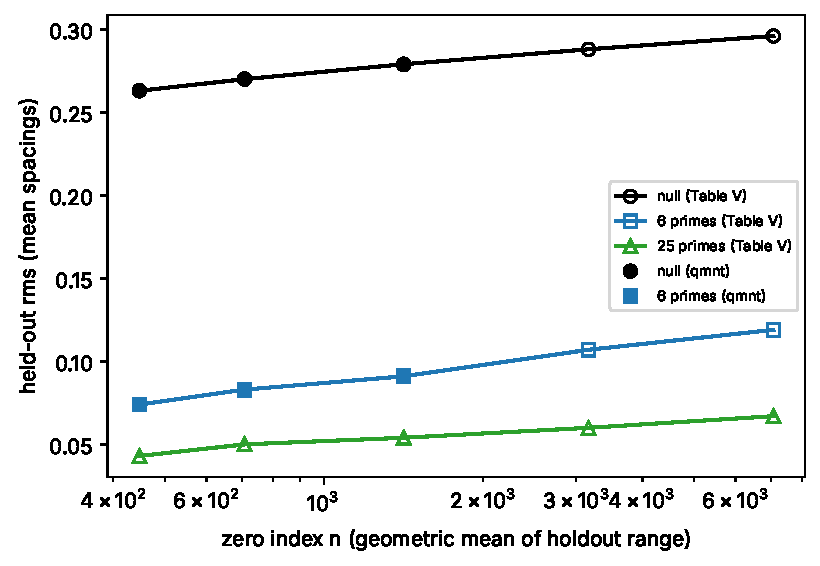
\includegraphics[width=0.85\linewidth]{figs/paper-critique_height.pdf}
\caption{Null rms and oracle rms (6 and 25 primes) as functions of height, in units of local mean spacing. Lines with open markers: paper Table~V for the five holdouts 401--500 through 5001--10000, plotted at the geometric mean of each index range. Filled markers: recomputed with \texttt{qmnt} for the holdouts up to zero 2000 (null and 6 primes). The null grows slowly with height. The oracle's error grows somewhat faster than the null: for six primes, $\mathcal S$ of \eqref{eq:paper-critique-skill} falls from $0.72$ to $0.60$ between the first and last holdout, and for 25 primes from $0.84$ to $0.77$. The Table~V caption describes this as nearly constant relative skill.}
\label{fig:paper-critique-height}
\end{figure}

\subsection{A leakage test you can run}

App.~A step 20 reports, for the sinusoidal controls, a simple but powerful check: overwrite the held-out data with noise, refit, and confirm that every fitted coefficient is bit-identical. If anything changes, held-out information leaked into the fit. Here is the test for a small version of control B (frequencies $m\log p$ given, amplitudes fitted by least squares, Chapter~\ref{ch:sparse-frequency}).

\begin{pycode}
import numpy as np, qmnt
t = qmnt.zeros(500).copy()
n = np.arange(1, 501)
train = n <= 400                            # training indices 1..400
P = qmnt.first_primes(3)
omegas = np.array([m * np.log(p) for p in P for m in (1, 2, 3)])

def fit(heights):
    y = n - 0.5 - qmnt.Nsm(heights)         # targets y_n of Sec. II D
    tt, yy = heights[train], y[train]       # training rows only
    X = np.hstack([np.sin(np.outer(tt, omegas)),
                   np.cos(np.outer(tt, omegas))])
    return np.linalg.lstsq(X, yy, rcond=None)[0]

c1 = fit(t)
rng = np.random.default_rng(0)
t_noisy = t.copy()
t_noisy[~train] = rng.uniform(0, 5000, size=100)   # destroy the holdout
c2 = fit(t_noisy)
print(np.array_equal(c1, c2))               # True: no leakage
\end{pycode}

The test is only as strong as what it overwrites: here the held-out heights. A pipeline that also reads held-out information from a second source (for example, a precomputed table of fluctuations) would need that source overwritten too.

\begin{keyideas}
\item The Zenodo record holds scripts, zeros, coefficients, logs and the parameter record; \texttt{run\_all.sh} reruns the pipeline.
\item Anchors ($t_1$, $t_{500}$, null $0.2631$, $L$ values, Table~V rows) are cheap first checks of any reconstruction.
\item Overwriting held-out data and checking bit-identical coefficients is a direct leakage test.
\end{keyideas}

%======================================================================
\section{How to go further: research projects}\label{sec:paper-critique-projects}

Each project below starts from a limit or open question of the paper. The rating is $\star$ (a weekend with \texttt{qmnt}), $\star\star$ (a few weeks; requires writing your own fitting loop from Chapter~\ref{ch:fitting}) or $\star\star\star$ (open-ended; could become a research paper). For each we state what success would look like. Any project that fits an operator should report the paper's four-item standard.

\paragraph{Project 1 ($\star$): extend Table~V.} Recompute the oracle rows with \texttt{qmnt} for 401--500, 501--1000 and 1001--2000, then for 2001--5000 and 5001--10000 (\texttt{qmnt.zeros} goes to $10^4$). Add 50 and 100 primes. Success: you reproduce the paper's rows and quantify how relative skill \eqref{eq:paper-critique-skill} depends on the prime budget.

\paragraph{Project 2 ($\star$): within-height kriging.} Reimplement the simple kriging interpolator of Sec.~III (App.~A step 19: autocovariance to lag 40, $\cos^2$ taper, positive-semidefinite projection, nugget $0.05$) on random 80/20 splits of zeros 1--400. Success: held-out correlation near the paper's $+0.87$, and the null on permuted targets.

\paragraph{Project 3 ($\star\star$): control C2 from scratch.} Implement the greedy sparse frequency search (Chapter~\ref{ch:sparse-frequency}) on 400 zeros, choosing $K$ by the forward split. List the selected frequencies, and for each compute $\bar m(\omega)$ from \eqref{eq:paper-critique-density}, so you can see which matches are individually informative.

\paragraph{Project 4 ($\star\star$): a small operator memorization study.} Using \texttt{qmnt.fit\_potential} (one call per run, slow), reproduce the qualitative shape of paper Fig.~3 at small $M$: in-sample error falling with $M$, held-out error at or above the null. Then refit to a permuted target (item (iv)).

\paragraph{Project 5 ($\star\star$): a Hermite basis.} Replace $\cos(k\pi x/L)$ by even Hermite functions $\phi_k(x)=H_{2k}(x/\ell)\,e^{-x^2/(2\ell^2)}$, the harmonic-oscillator eigenfunctions of Chapter~\ref{ch:bound-states} (up to normalization) with a length scale $\ell$ you choose. Here $H_j$ is the Hermite polynomial of degree $j$. It is defined by $H_0(u)=1$, $H_1(u)=2u$ and the recurrence $H_{j+1}(u)=2uH_j(u)-2jH_{j-1}(u)$; for example, $H_2(u)=4u^2-2$. \texttt{scipy.special.eval\_hermite} evaluates these polynomials. Write the Gauss--Newton loop of Chapter~\ref{ch:fitting} with this basis. Success: an honest table in the format of paper Table~II, with bootstrap intervals. This tests one of the parametrizations the paper names as untested.

\paragraph{Project 6 ($\star\star\star$): a neural-network potential.} Represent $\delta V(x)$ by a small neural network (a composition of linear maps and a fixed nonlinear function) and fit its weights. The paper names this as untested. The difficulty is not the code but the protocol: report restarts, regularization, and surrogates exactly as for the other bases.

\paragraph{Project 7 ($\star\star$): another background.} Replace the Wu--Sprung background by a different even confining potential (for example one whose WKB levels track $s_n$ only approximately, to test sensitivity to the background), or add Wu and Sprung's fractal corrections~\cite{wusprung} to the background. Recompute the turning-point map (\cref{fig:paper-critique-turning}) first, then rerun the held-out protocol.

\paragraph{Project 8 ($\star\star$): rerun Sec.~V at small scale.} On a small grid, compute the second-order tensors of paper Eq.~(5) for a PT-odd basis, fit, and compare with exact complex diagonalization at full and quarter amplitude. Check the exact sum rule \eqref{eq:paper-critique-trace}. This addresses Limit 4.

\paragraph{Project 9 ($\star\star\star$): higher zeros.} Operator fits stopped at zero 1000 and fitted controls were scored below zero 2000. Extend the controls to zeros near $10^4$ with \texttt{qmnt}, and think about how the cost of operator fits grows with the number of levels (the grid must resolve the local wavelength $\pi/\sqrt E$, Chapter~\ref{ch:fitting}). Zeros much higher than $10^4$ can be computed with \texttt{mpmath} slowly, or taken from the tables of zeros that Odlyzko has made publicly available. These tables are not the cited paper; his study of spacings is~\cite{odlyzko87}.

\paragraph{Project 10 ($\star\star\star$, open): derive the memorization result.} In the linearized regime of Chapter~\ref{ch:perturbation}, a fit with training sensitivity matrix $A_{\rm in}$ (rows: training levels) and held-out sensitivity $A_{\rm out}$ predicts held-out shifts $A_{\rm out}\,A_{\rm in}^{+}\,r_{\rm in}$, where $A_{\rm in}^{+}$ is the (regularized) pseudo-inverse of Chapter~\ref{ch:least-squares} and $r_{\rm in}$ the training residuals. Skill requires this ``transfer matrix'' $A_{\rm out}A_{\rm in}^{+}$ to map true training fluctuations to true held-out ones. Compute it for the cosine basis on the Wu--Sprung background and study its structure. The paper calls the derivation an open problem; a convincing first-order analysis would be a contribution.

\paragraph{Project 11 ($\star\star\star$): Dirichlet $L$-functions.} The zeta function is one member of a family. For the character $\chi_4$ modulo 4 ($\chi_4(k)=0$ for even $k$, $1$ for $k\equiv1$, $-1$ for $k\equiv3 \pmod 4$), the function $L(s,\chi_4)=\sum_k\chi_4(k)k^{-s}$ has its own zeros and its own explicit formula, in which each prime term is weighted by $\chi_4(p)^m$. \texttt{mpmath} evaluates such functions (\texttt{mpmath.dirichlet}); you must locate zeros yourself by sign changes of a suitable real function and Brent's method, and look up the smooth counting function in a number theory text such as~\cite{davenport}. Then repeat the oracle-versus-fit comparison. Success: the paper's protocol transferred to a second spectrum.

\begin{keyideas}
\item Projects 1--4 reproduce and vary the paper's results; 5--8 test what the paper names as untested; 9--11 extend its scope; Project 10 attacks its stated open problem.
\item Any operator fit you report should satisfy the four-item standard of \cref{sec:paper-critique-standard}.
\end{keyideas}

%======================================================================
\section{Paper connection}\label{sec:paper-critique-paper}

This chapter is itself a reading of the paper, so the connection is a map from our sections to R1's numbering.

\begin{table}[htbp]\centering\small
\caption{Where each part of this chapter meets the paper (R1 numbering).}
\label{tab:paper-critique-connection}
\begin{tabular}{p{4.3cm}p{8.4cm}}
\toprule
This chapter & Paper \\
\midrule
\Cref{sec:paper-critique-claims}, scope & Sec.~VI para.~1; Sec.~I scope paragraph; Sec.~I~A~d \\
\Cref{sec:paper-critique-claims}, heuristic & Sec.~VI para.~2; Sec.~III (coverage, surrogates, interpolation split, Fig.~4, continuation probe); Table~III; Table~IV \\
Relative skill, best rescaling & Tables~I, IV, V; Fig.~1 (corr $-0.07$ vs $+0.96$) \\
Coverage threshold & Sec.~III first paragraph; Table~I scale-2 rows; App.~A key anchors \\
\Cref{sec:paper-critique-standard} & Sec.~VI para.~5; items motivated by Fig.~1, Tables~I, III; Sec.~V and Fig.~5; Table~I ridge rows and caption; Sec.~III surrogates \\
\Cref{sec:paper-critique-limits} & Sec.~VI para.~3; Table~II (Chebyshev $M=400$); Sec.~IV dephasing ($0.078$/$+0.96$); Sec.~III block bootstrap; App.~A steps 13, 22 \\
W1 & Sec.~I~A~a; App.~A literature audit \\
W2, W3 & Sec.~II~B, Eq.~(2), $L$ values; Sec.~III interpolation split; Fig.~4 \\
W4 & Sec.~V, V~A, Eq.~(5), Fig.~5; App.~A steps 9--11 \\
W5 & Sec.~IV (alignment, surrogate check); App.~A steps 20, 23; refs.~\cite{landau,gonek} \\
W8, W9 & Captions of Tables~I, III, IV; Sec.~II~C two nulls; Sec.~II~F \\
\Cref{sec:paper-critique-repro} & Data Availability; App.~A steps 1--23 and key anchors; Eqs.~(1), (3), (4); Table~V \\
\Cref{sec:paper-critique-projects} & Sec.~VI limits and open problem; untested bases named in Sec.~I and VI \\
\bottomrule
\end{tabular}
\end{table}

Three points deserve emphasis. First, the paper's own hedges are its strongest feature: ``heuristically'', ``exploratory'', ``not excluded'', ``within the operator families tested''. When you summarize the paper, keep them. Second, the paper's novelty claim is the controlled out-of-sample comparison and the protocol, not the explicit formula, which it attributes to the classical Riemann--von Mangoldt/Guinand--Weil theory and to Fran\c{c}a and LeClair~\cite{francaleclair,leclair}. Third, the falsifiability standard (Sec.~VI) is the part of the paper most likely to outlast its specific numbers: it is a checklist anyone can apply to the next claim of a fitted ``zeta operator''.

%======================================================================
\section{Summary}\label{sec:paper-critique-summary}

\begin{itemize}
\item Sec.~VI of the paper constrains only an empirical shortcut, not the analytic Hilbert--P\'olya program; its explanation of the failure is heuristic, and whether memorization can be derived is open (\cref{tab:paper-critique-status}).
\item Relative skill $\mathcal{S}=1-\text{rms}/\text{null}$, \eqref{eq:paper-critique-skill}: $-0.40$ for the $M=400$ operator and $+0.72$ for the six-prime oracle on zeros 401--500.
\item The best rms obtainable by rescaling a prediction with correlation $r$ is null$\times\sqrt{1-r^2}$; uncorrelated predictions cannot beat the null.
\item Coverage threshold $M>2\sqrt EL/\pi$: about 814 at scale 1 and about 1313 for the top training levels at scale 2.
\item The proposed standard: (i) held-out rms and corr against the model's own null, including a within-height split; (ii) exact spectra; (iii) robustness to regularization and restarts; (iv) surrogate refits. It is necessary, not sufficient.
\item Multiple comparisons, \eqref{eq:paper-critique-atleastone}: one marginal row in eight is expected about one time in five under rough independence.
\item Dephasing, \eqref{eq:paper-critique-dephase}: phase error $m\,\delta\omega\,(t-t_*)$ grows linearly with distance from the window.
\item Rule of three, \eqref{eq:paper-critique-rule3}: ``none of $n$'' bounds a per-item rate by about $3/n$.
\item Exact sum rule, \eqref{eq:paper-critique-trace}: real shifts of $H+iA$ sum to zero at all orders over a finite basis.
\item Chance alignment, \eqref{eq:paper-critique-density}: expected number of primes within $\pi/T$ of $\omega$ is about $(2\pi/T)e^\omega/\omega$; near $\omega=8$ chance matches are almost certain.
\item Anchors and a Table~V row are reproducible with \texttt{qmnt}; a leakage test compares coefficients after overwriting held-out data.
\end{itemize}

%======================================================================
\section{Problems}\label{sec:paper-critique-problems}

\begin{problemlist}
\prob{1}{List the four items of the falsifiability standard proposed in Sec.~VI of the paper. For each, name one experiment in the paper (section, table or figure) that shows why the item is needed.}

\prob{1}{Using \eqref{eq:paper-critique-skill} with null $0.263$, compute the relative skill on zeros 401--500 of: the $M=600$ cosine operator (OOS $0.313$, Table~I), control C1 ($0.258$, Table~IV), and control B with 25 primes ($0.028$, Table~IV).}

\prob{1}{The interpolation split (Sec.~III) has gap error $2.64$ spacings against a null of $0.255$. Compute the ratio and compare with the paper's phrase ``ten times the null''.}

\prob{1}{Classify each statement as (A) a limit the paper states in Sec.~VI, (B) a weak point a referee could raise that is not among the Sec.~VI limits, or (C) a claim the paper does not make: (a) Hermite bases were not tested. (b) The literature-gap claim rests on a keyword search of two citation lists. (c) The truncated explicit formula is a new result. (d) Sec.~V was not rerun for the revision.}

\prob{1}{From the Data Availability statement, list what the Zenodo record contains, and give the DOI of the version as first submitted.}

\prob{1}{Check the paper's claim (Sec.~IV) that one prime beats every fitted operator's holdout performance by a factor $\gtrsim1.3$. Use the two lowest-rms operator rows scored on 401--500, Table~I ridge $\mu=0.3$ (OOS $0.265$) and Table~II Chebyshev ridge $\mu=0.3$ (OOS $0.264$), and compare them with the one-prime oracle ($0.198$, Table~V). Why does this check not cover every operator row in Table~I?}

\prob{2}{In the arithmetic-continuation probe (Sec.~III; App.~A anchors), the OOS rms is $0.1958$ against a probe-null of $0.1708$. By what percentage is the fit worse than predicting zero fluctuation? Why is the probe-null smaller than the real-zero null $0.263$?}

\prob{2}{For the amplitude-controlled $R=4$ fits of Sec.~V, the exact-verified in-sample rms values are $0.2391$ (odd) and $0.2423$ (even), against the null $0.2438$. Compute the percentage gains and compare with the paper's $1.9\%$ and $0.6\%$.}

\prob{2}{Table~I has twelve configurations. Using \eqref{eq:paper-critique-atleastone} with $\alpha=0.025$, find the probability that at least one would show a spuriously ``significant'' positive correlation if all had true correlation zero and were independent. Which assumption is most clearly violated?}

\prob{2}{Using \texttt{qmnt}, compute the null rms on zeros 401--500 and 501--1000 and compare with Table~V.}

\prob{2}{Using \texttt{qmnt}, reproduce the $\{2\}$ and 3-prime oracle entries of Table~V on zeros 401--500. Then compute the relative skill of each.}

\prob{2}{Using \texttt{qmnt.smooth\_zeros} and \texttt{qmnt.wu\_sprung\_x}, find the band of turning points of levels 401--500 (the principal holdout) in the Wu--Sprung potential. Express its ends as fractions of $L=44.883$.}

\prob{2}{In the dephasing sample, at what distance $t-t_*$ beyond the window does the worst-case phase error of the fundamental reach $\pi/2$? Express your answer in terms of $T$ and evaluate it for $T=666$, the window of zeros 1--400.}

\prob{2}{Using \eqref{eq:paper-critique-density} with $T=666$, compute the expected number of primes within $\pi/T$ of $\omega=3$ and $\omega=6$, and the probability of at least one.}

\prob{2}{Choose your own $E=(E_1,E_2,E_3)$ with distinct values and a real symmetric $3\times3$ matrix $A$ with nonzero diagonal. Compute the second-order real shifts from paper Eq.~(5) and verify that they sum to zero. Then diagonalize $\mathrm{diag}(E)+iA$ with \texttt{numpy.linalg.eigvals} and verify \eqref{eq:paper-critique-trace}.}

\prob{2}{Explain in your own words why item (i) of the standard requires a within-height split, using the growth of the null in Table~V and the results of Table~III.}

\prob{2}{Design a leakage test, in the style of the listing in \cref{sec:paper-critique-repro}, for control C2. What exactly must be overwritten, and which outputs must be identical?}

\prob{2}{Sec.~III reports surrogate in-sample rms $0.134\pm0.010$ (permuted), $0.141\pm0.006$ (phase-randomized), $0.138\pm0.005$ (amplitude-adjusted), against $0.137$ on the true zeros. Assuming each $\pm$ is the spread over ten draws, by how many spreads does the true-zero value differ from each surrogate mean? What do you conclude?}

\prob{2}{The scale-2 $M=300$ row of Table~I required a relaxed step-acceptance threshold. Explain why the paper calls it a ``sensitivity result'', and why including it does not change the qualitative conclusion.}

\prob{3}{Using \texttt{qmnt}, form the odd/even split of zeros 1--400 and predict each held-out fluctuation by the mean of its two nearest training fluctuations. Compute the correlation with the truth and compare with the paper's range $-0.26$ to $-0.41$ (Sec.~III, within-height splits). Explain the sign using the negative autocorrelation at lags 1--3.}

\prob{3}{The six primes between 131 and 211 selected by the 800-zero C2 fit lie at $\omega\approx4.9$--$5.4$. For the 800-zero window, $T=t_{800}-t_1\approx1170$. Compute $\bar m(\log131)$ from \eqref{eq:paper-critique-density} and the probability of a chance match. Write two sentences, as a referee, on what this does and does not imply for the paper's alignment claim.}

\prob{3}{Using \texttt{qmnt} and the circular block bootstrap of Chapter~\ref{ch:controls}, compute 95\% intervals for the six-prime oracle's held-out correlation on 401--500 with block lengths 1, 5 and 20. Compare with the paper's $[+0.95,+0.97]$.}

\prob{3}{Connes~\cite{connes26} obtains approximations to the first 50 zeros from primes $p\le13$ alone. Explain why the paper says that for this construction ``no held-out evaluation question arises'', and describe what test is appropriate instead.}

\prob{3}{(Research.) For a small grid and the cosine basis with $M=50$, compute the first-order sensitivity matrices $A_{\rm in}$ (levels 1--40) and $A_{\rm out}$ (levels 41--50) of the unperturbed Wu--Sprung potential using \texttt{qmnt.fd\_levels} with \texttt{return\_vectors=True}. Form the transfer matrix $A_{\rm out}A_{\rm in}^{+}$ with a small ridge. Apply it to the true training fluctuations and compute the correlation of its output with the true held-out fluctuations. Discuss.}

\prob{3}{Extend the rule-of-three sample: suppose the keyword search detects a relevant work with probability $d=0.8$ (it misses 20\%). With $n=29$ works and none detected, find the 95\% upper bound on the per-work rate $f$ of held-out tests.}

\end{problemlist}

%======================================================================
\section{Answers to selected problems}\label{sec:paper-critique-answers}

\textbf{Problem 1.} (i) Train/test split with held-out rms and corr against the model's own null, including a within-height split: Fig.~1 and Table~I (forward splits), Table~III (within-height splits, needed because the null grows with height, Table~V). (ii) Score the exact operator spectrum: Sec.~V and Fig.~5, where the second-order surrogate floor $0.232$ became $0.2523$ (worse than the null) under exact diagonalization. (iii) Survival under regularization and restarts: Table~I ridge rows and random-init repeats (caption), and the interpolation split under ridge (Sec.~III). (iv) Refit to permuted and phase-randomized targets: Sec.~III, where surrogates are fitted as well as the true zeros.

\textbf{Problem 2.} $\mathcal S=1-0.313/0.263=1-1.190=-0.190$ (operator worse than the null); $\mathcal S=1-0.258/0.263=1-0.981=+0.019$ (C1 essentially at the null); $\mathcal S=1-0.028/0.263=1-0.106=+0.894$ (B with given frequencies predicts well).

\textbf{Problem 3.} $2.64/0.255=10.35$. ``Ten times'' is accurate. (With the anchor $2.6434$ the ratio is $10.37$.)

\textbf{Problem 4.} (a) A: stated in Sec.~VI para.~3. (b) B: the audit is recorded in App.~A but its limits are not listed in Sec.~VI. (c) C: the paper explicitly claims no novelty for the formula. (d) A: stated in Sec.~VI para.~3.

\textbf{Problem 5.} All scripts, computed zeros, fitted coefficients, and the full parameter record of App.~A; for the revision, the scripts, coefficients, logs and result files of steps 16--23, with an audit file mapping them. The first-submission version has DOI 10.5281/zenodo.21842988.

\textbf{Problem 6.} $0.265/0.198=1.34$ and $0.264/0.198=1.33$. Both are consistent with ``$\gtrsim1.3$'', narrowly. The other Table~I rows are scored on different holdouts (and the scale-2 rows with a different null). Checking them would need the one-prime oracle on exactly those holdouts, which Table~V does not list, so the check covers only the rows scored on 401--500. You could compute the missing one-prime values yourself with \texttt{qmnt.oracle\_zeros}.

\textbf{Problem 7.} $(0.1958-0.1708)/0.1708=0.0250/0.1708=0.146$, so the fit is about $14.6\%$ worse than predicting zero fluctuation. The probe-null is the rms of the synthetic target itself, which contains only the $p=2$ terms ($m\le3$). The real fluctuations also contain the contributions of all other primes, so their rms is larger.

\textbf{Problem 8.} Odd: $(0.2438-0.2391)/0.2438=0.0047/0.2438=0.0193$, i.e. $1.93\%$. Even: $(0.2438-0.2423)/0.2438=0.0015/0.2438=0.0062$, i.e. $0.62\%$. Both round to the paper's $1.9\%$ and $0.6\%$.

\textbf{Problem 9.} By \eqref{eq:paper-critique-atleastone}, $1-0.975^{12}=1-0.738=0.262$. The most clearly violated assumption is independence. The rows share training and held-out zeros, and several differ only in $M$ or in the ridge strength, so their errors are strongly related.

\textbf{Problem 10.} Compute \texttt{qmnt.rms(qmnt.fluct(t[n-1], n))} for \texttt{n = np.arange(401, 501)} and \texttt{np.arange(501, 1001)}. You obtain $0.263$ and $0.270$, the Table~V nulls.

\textbf{Problem 11.} Run the Table~V listing of \cref{sec:paper-critique-repro} with $k=1$ and $k=3$. The results are rms $0.198$, corr $+0.66$ and rms $0.116$, corr $+0.90$, the Table~V entries. Relative skill: $1-0.198/0.263=0.247$ and $1-0.116/0.263=0.559$.

\textbf{Problem 12.} $s_{401}\approx681$ and $s_{500}\approx811$, giving $x(s_{401})\approx33.9$ and $x(s_{500})\approx38.5$. As fractions of $L$: $33.9/44.883=0.755$ and $38.5/44.883=0.858$. The principal holdout probes a band in the outer quarter of the box, beyond the interpolation-gap band $22.5$--$28.5$.

\textbf{Problem 13.} The phase error of the fundamental is $\delta\omega\,(t-t_*)$ with $\delta\omega=\pi/T$. Setting it equal to $\pi/2$ gives $(\pi/T)(t-t_*)=\pi/2$, so $t-t_*=T/2$. For $T=666$ this is $333$ in $t$.

\textbf{Problem 14.} $2\pi/666=0.009434$. At $\omega=3$: $e^3/3=6.695$, $\bar m=0.0632$, $P=1-e^{-0.0632}=0.061$. At $\omega=6$: $e^6/6=67.24$, $\bar m=0.634$, $P=1-e^{-0.634}=0.470$.

\textbf{Problem 15.} One example: $E=(1,2,4)$, and $A$ with diagonal $(0.3,-0.4,0.1)$ and off-diagonal entries $A_{12}=0.2$, $A_{13}=-0.1$, $A_{23}=0.25$. The diagonal does not enter Eq.~(5), because the sum excludes $m=n$; it gives only the imaginary first-order shifts $iA_{nn}$. Eq.~(5) gives
\begin{align*}
\delta E_1&=-[0.04/(-1)+0.01/(-3)]=0.04333,\\
\delta E_2&=-[0.04/1+0.0625/(-2)]=-0.00875,\\
\delta E_3&=-[0.01/3+0.0625/2]=-0.03458.
\end{align*}
These sum to zero, because each pair $(n,m)$ contributes $-A_{nm}^2/(E_n-E_m)$ to level $n$ and the opposite amount to level $m$. The real parts of the exact eigenvalues sum to $7=1+2+4$, as \eqref{eq:paper-critique-trace} requires: the trace is $7+i(0.3-0.4+0.1)=7$.

\textbf{Problem 16.} In a forward split the held-out zeros are higher, where the fluctuation amplitude is larger (null $0.263$ on 401--500 rising to $0.296$ on 5001--10000, Table~V). A model could fail because the test data differ in distribution (covariate shift) rather than because it captured no structure. A split within one height range removes the shift. Table~III shows the fits fail even then (for the random 80/20 splits, held-out errors $1.5$--$3.0$ times the null at scale 1), so covariate shift is not the explanation, while kriging and the oracle succeed on the same held-out sets, showing that predictable structure is present.

\textbf{Problem 17.} Overwrite every held-out height (all zeros beyond the training window) with noise. Also overwrite any other source of held-out information, such as a precomputed table of fluctuations. Then rerun the \emph{complete} C2 procedure: the periodogram search, the forward split inside the training window that chooses $K$ and the ridge strength, and the final refit on the whole window. The number $K$, the selected frequencies, the chosen ridge strength and all fitted amplitudes must be bit-identical to those from the clean run. Comparing only the final amplitudes would miss leakage into the model-selection step.

\textbf{Problem 18.} Permuted: $(0.137-0.134)/0.010=0.3$. Phase-randomized: $(0.141-0.137)/0.006=0.67$. Amplitude-adjusted: $(0.138-0.137)/0.005=0.2$. All differences are well under one spread: the fit does no better on the real zeros than on targets with no arithmetic content, so in-sample accuracy measures capacity.

\textbf{Problem 19.} Under the strict acceptance rule (an improvement factor of $0.999$, App.~A step 6), the optimizer accepts no step for this configuration. The fitted potential therefore stays at $c=0$, which is the null. To obtain a fitted row at all, the threshold was relaxed to $1-10^{-5}$ for this row only. A result that exists only after changing one setting of the protocol measures how sensitive the outcome is to that setting; it is not a default-protocol result, hence ``sensitivity result''. Including it does not change the conclusion. The relaxed fit scores OOS $0.370$ with corr $-0.01$, worse than the null $0.274$, and the strict fit is at the null. Neither shows skill.

\textbf{Problem 21.} $\log131=4.875$, $e^{4.875}/4.875=131/4.875=26.87$, $2\pi/1170=0.005370$, so $\bar m=0.144$ and $P=1-e^{-0.144}=0.134$. Referee: a single match near $\omega\approx4.9$ has roughly a one-in-seven chance of occurring by accident, so no single high-frequency match is strong evidence. The claim rests instead on the collective alignment compared with a surrogate ensemble, which the paper reports and labels exploratory; and C2's held-out predictive skill stands independently of the alignment statistic.

\textbf{Problem 23.} The construction takes only prime data as input; no zero is used to fit anything. There is no training set, so every zero is effectively held out and the question of transfer from training to test does not arise. The appropriate test is direct: compare the constructed values with the true zeros (the paper reports accuracies from $10^{-3}$ down to $2.6\times10^{-55}$) and check the mathematical guarantees (location on the critical line).

\textbf{Problem 25.} A relevant work is detected with probability $fd$. Then $(1-fd)^{n}=0.05$ gives $fd=1-0.05^{1/29}=0.0981$, so $f=0.0981/0.8=0.123$. Keyword misses loosen the bound from about 10\% to about 12\% per work.
